\documentclass[12pt]{report}
\usepackage[utf8]{inputenc}
\usepackage[russian]{babel}
%\usepackage[14pt]{extsizes}
\usepackage{listings}
\usepackage{graphicx}
\usepackage{amsmath,amsfonts,amssymb,amsthm,mathtools} 
\usepackage{pgfplots}
\usepackage{filecontents}
\usepackage{indentfirst}
\usepackage{eucal}
\usepackage{amsmath}
\usepackage{enumitem}
\frenchspacing

\usepackage{indentfirst} % Красная строка


%\usetikzlibrary{datavisualization}
%\usetikzlibrary{datavisualization.formats.functions}

\usepackage{amsmath}




% Для листинга кода:
\lstset{ %
language=haskell,                 % выбор языка для подсветки (здесь это С)
basicstyle=\small\sffamily, % размер и начертание шрифта для подсветки кода
numbers=left,               % где поставить нумерацию строк (слева\справа)
numberstyle=\tiny,           % размер шрифта для номеров строк
stepnumber=1,                   % размер шага между двумя номерами строк
numbersep=5pt,                % как далеко отстоят номера строк от подсвечиваемого кода
showspaces=false,            % показывать или нет пробелы специальными отступами
showstringspaces=false,      % показывать или нет пробелы в строках
showtabs=false,             % показывать или нет табуляцию в строках
frame=single,              % рисовать рамку вокруг кода
tabsize=2,                 % размер табуляции по умолчанию равен 2 пробелам
captionpos=t,              % позиция заголовка вверху [t] или внизу [b] 
breaklines=true,           % автоматически переносить строки (да\нет)
breakatwhitespace=false, % переносить строки только если есть пробел
escapeinside={\#*}{*)}   % если нужно добавить комментарии в коде
}

\usepackage[left=2cm,right=2cm, top=2cm,bottom=2cm,bindingoffset=0cm]{geometry}
% Для измененных титулов глав:
\usepackage{titlesec, blindtext, color} % подключаем нужные пакеты
\definecolor{gray75}{gray}{0.75} % определяем цвет
\newcommand{\hsp}{\hspace{20pt}} % длина линии в 20pt
% titleformat определяет стиль
\titleformat{\chapter}[hang]{\Huge\bfseries}{\thechapter\hsp\textcolor{gray75}{|}\hsp}{0pt}{\Huge\bfseries}


% plot
\usepackage{pgfplots}
\usepackage{filecontents}
\usetikzlibrary{datavisualization}
\usetikzlibrary{datavisualization.formats.functions}

\begin{document}
\setcounter{page}{2}
\tableofcontents

\newpage
\chapter*{Введение}
\addcontentsline{toc}{chapter}{Введение}
Ускорение вычислительных алгоритмов с использованием программируемых логических интегральных схем (ПЛИС) имеет ряд преимуществ по сравнению с их реализацией на универсальных микропроцессорах, или графических процессорах. В то время, как традиционная разработка программного обеспечения связана с программированием на заранее определенном наборе машинных команд, разработка программируемых устройств - это создание специализированной вычислительной структуры для реализации желаемой функциональности.

Микропроцессоры и графические процессоры имеют предопределенную архитектуру с фиксированным количеством ядер, набором инструкций, и жесткой архитектурой памяти, и обладают высокими тактовыми частотами и хорошо сбалансированной конвейерной структурой. Графические процессоры масштабируют производительность за счет большого количества ядер и использования параллелизма SIMD/SIMT (Рисунок 1). В отличие от них, программируемые устройства представляют собой полностью настраиваемую архитектуру, которую разработчик может использовать для размещения вычислительных блоков с требуемой функциональностью. В таком случает, высокий уровень производительности достигается за счет создания длинных конвейеров обработки данных, а не за счет увеличения количества вычислительных единиц. Понимание этих преимуществ является необходимым условием для разработки вычислительных устройств и достижения наилучшего уровня ускорения.

\textbf{Цель работы}: Изучение методики и технологии синтеза аппаратных устройств ускорения вычислений по описаниям на языках высокого уровня. В ходе лабораторной работы рассматривается маршрут проектирования устройств, представленных в виде синтаксических конструкций ЯВУ C/C++, изучаются принципы работы IDE Xilinx Vitis HLS и методика анализа и отладки устройств. Для достижения данной цели необходимо выполнить следующие задачи:
\begin{itemize}
\item разработать ускоритель вычислений по индивидуальному заданию;
\item разработать код для тестирования ускорителя;
\item реализовать ускоритель с помощью средств высоко-уровненного синтеза;
\item выполнить отладку ускорителя.
\end{itemize}

Все задания выполняются в соответствии с \textbf{вариантом №4}.

\chapter{Сборка и отладка проекта в режиме программной эмуляции (Emulation-SW)}

Функции ядра на основе индивидуального задания с использованием не оптимизированного цикла, конвейерного цикла, частично развернутого цикла и конвейерного, частично развернутого цикла приведены в листингах \ref{lst:no_pragmas}, \ref{lst:pipelined}, \ref{lst:unrolled} и \ref{lst:pipe_unroll} соответственно.

\begin{lstlisting}[label=lst:no_pragmas,caption=Не оптимизированный цикл]
extern "C" {
void var004_no_pragmas(int* c, const int* a, const int* b, const int len) {
    for (int x = 0; x < len; ++x) {
        int sumA = 0;
        int sumB = 0;
        int volA = a[x];
        int volB = b[x];
        for (int i = 0; i < 32; i++) {
            sumA += (volA) & 1;
            volA = volA/2;
            sumB += (volB) & 1;
            volB = volB/2;
        }
        if (sumA > sumB)
            c[x] = sumA;
        else
            c[x] = sumB;

    }
}
}
\end{lstlisting}

\newpage
\begin{lstlisting}[label=lst:pipelined,caption=Конвейерная организация цикла]
extern "C" {
void var004_pipelined(int* c, const int* a, const int* b, const int len) {
    for (int x = 0; x < len; ++x) {
	#pragma HLS PIPELINE
        int sumA = 0;
        int sumB = 0;
        int volA = a[x];
        int volB = b[x];
        for (int i = 0; i < 32; i++) {
	    #pragma HLS PIPELINE
            sumA += (volA) & 1;
            volA = volA/2;
            sumB += (volB) & 1;
            volB = volB/2;
        }
        if (sumA > sumB)
            c[x] = sumA;
        else
            c[x] = sumB;

    }
}
}
\end{lstlisting}

\begin{lstlisting}[label=lst:unrolled,caption=Частично развернутый цикл]
extern "C" {
void var004_unrolled(int* c, const int* a, const int* b, const int len) {
    for (int x = 0; x < len; ++x) {
        #pragma HLS UNROLL factor=2
        int sumA = 0;
        int sumB = 0;
        int volA = a[x];
        int volB = b[x];
        for (int i = 0; i < 32; i++) {
            sumA += (volA) & 1;
            volA = volA/2;
            sumB += (volB) & 1;
            volB = volB/2;
        }
        if (sumA > sumB)
            c[x] = sumA;
        else
            c[x] = sumB;

    }
    
}
}
\end{lstlisting}

\begin{lstlisting}[label=lst:pipe_unroll,caption=Конвейерный и частично развернутый цикл]
extern "C" {
void var004_pipe_unroll(int* c, const int* a, const int* b, const int len) {
    for (int x = 0; x < len; ++x) {
        #pragma HLS PIPELINE
        #pragma HLS UNROLL factor=2
        int sumA = 0;
        int sumB = 0;
        int volA = a[x];
        int volB = b[x];
        for (int i = 0; i < 32; i++) {
            sumA += (volA) & 1;
            volA = volA/2;
            sumB += (volB) & 1;
            volB = volB/2;
        }
        if (sumA > sumB)
            c[x] = sumA;
        else
            c[x] = sumB;

    }
}
}
\end{lstlisting}
Результаты запуска приложения, которые были выданы на вкладку Console в режиме Emulation-SW приведены на рисунке \ref{img:test_sw}.
\begin{figure}[h!p]
	\centering
	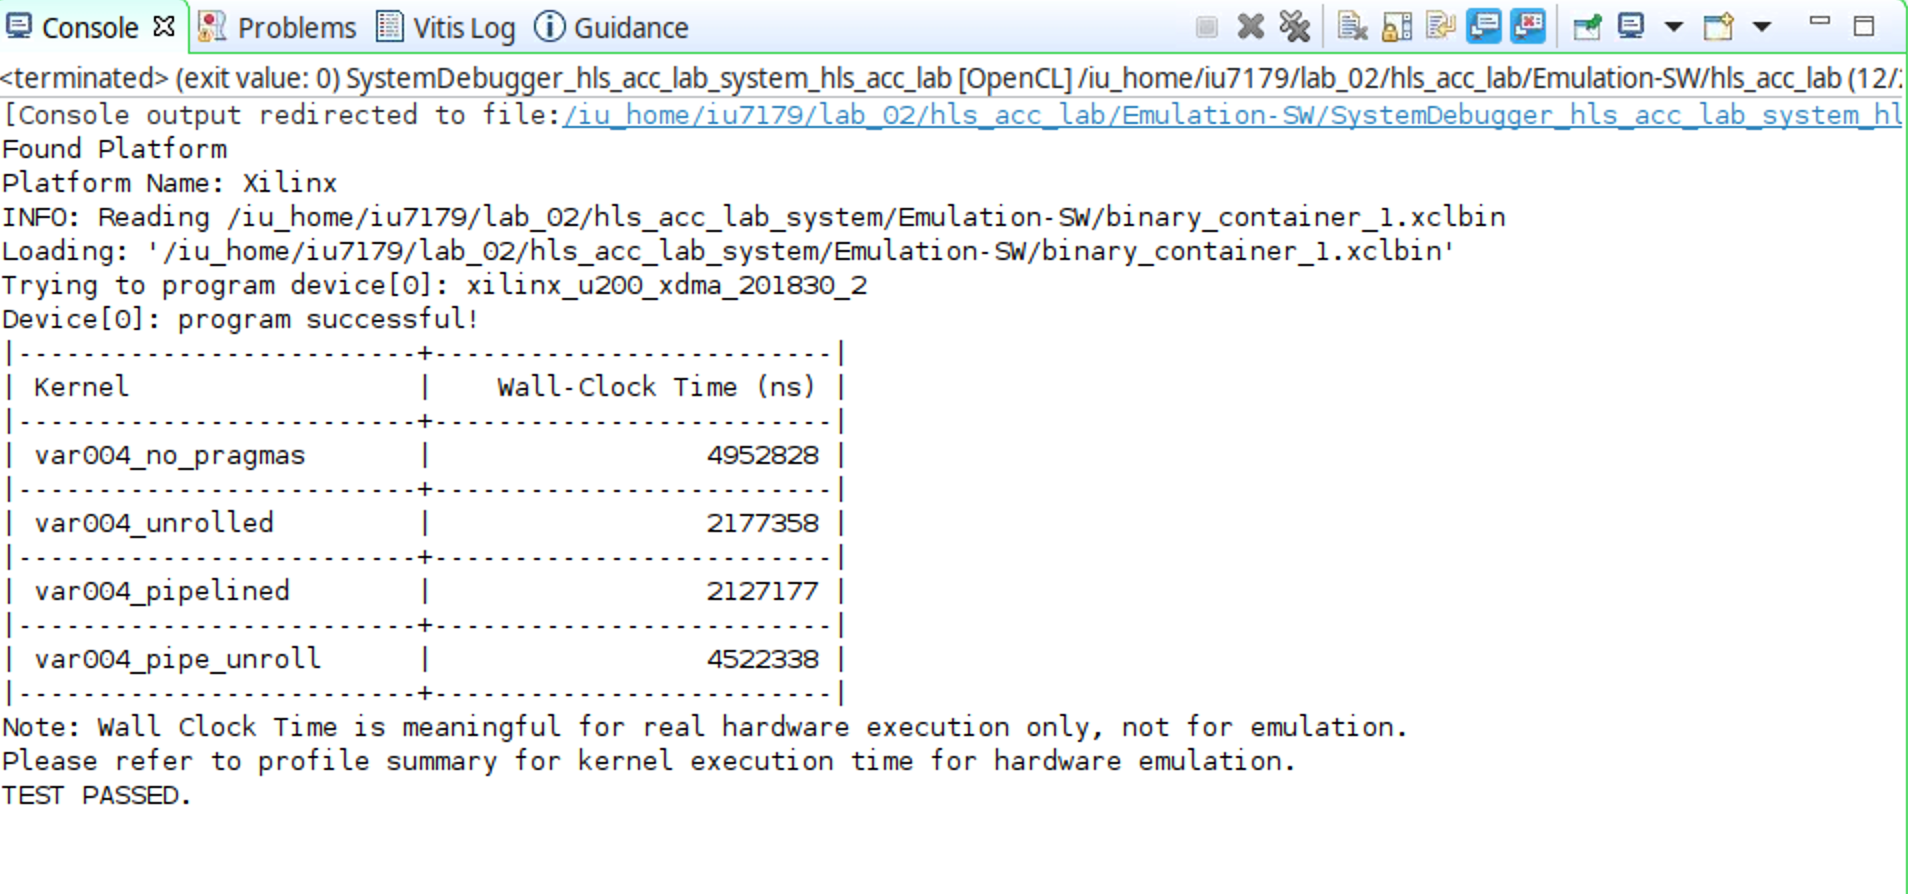
\includegraphics[width = \linewidth]{test_sw.png}
	\caption{Результаты запуска приложения в режиме Emulation-SW}
	\label{img:test_sw}
\end{figure}

\chapter{Сборка и отладка проекта в режиме аппаратной эмуляции (Emulation-HW)}
Копия экрана Assistant View для сборки Emulation-HW приведена на рисунках \ref{img:aview_1} и \ref{img:aview_2}.
\begin{figure}[h!p]
	\centering
	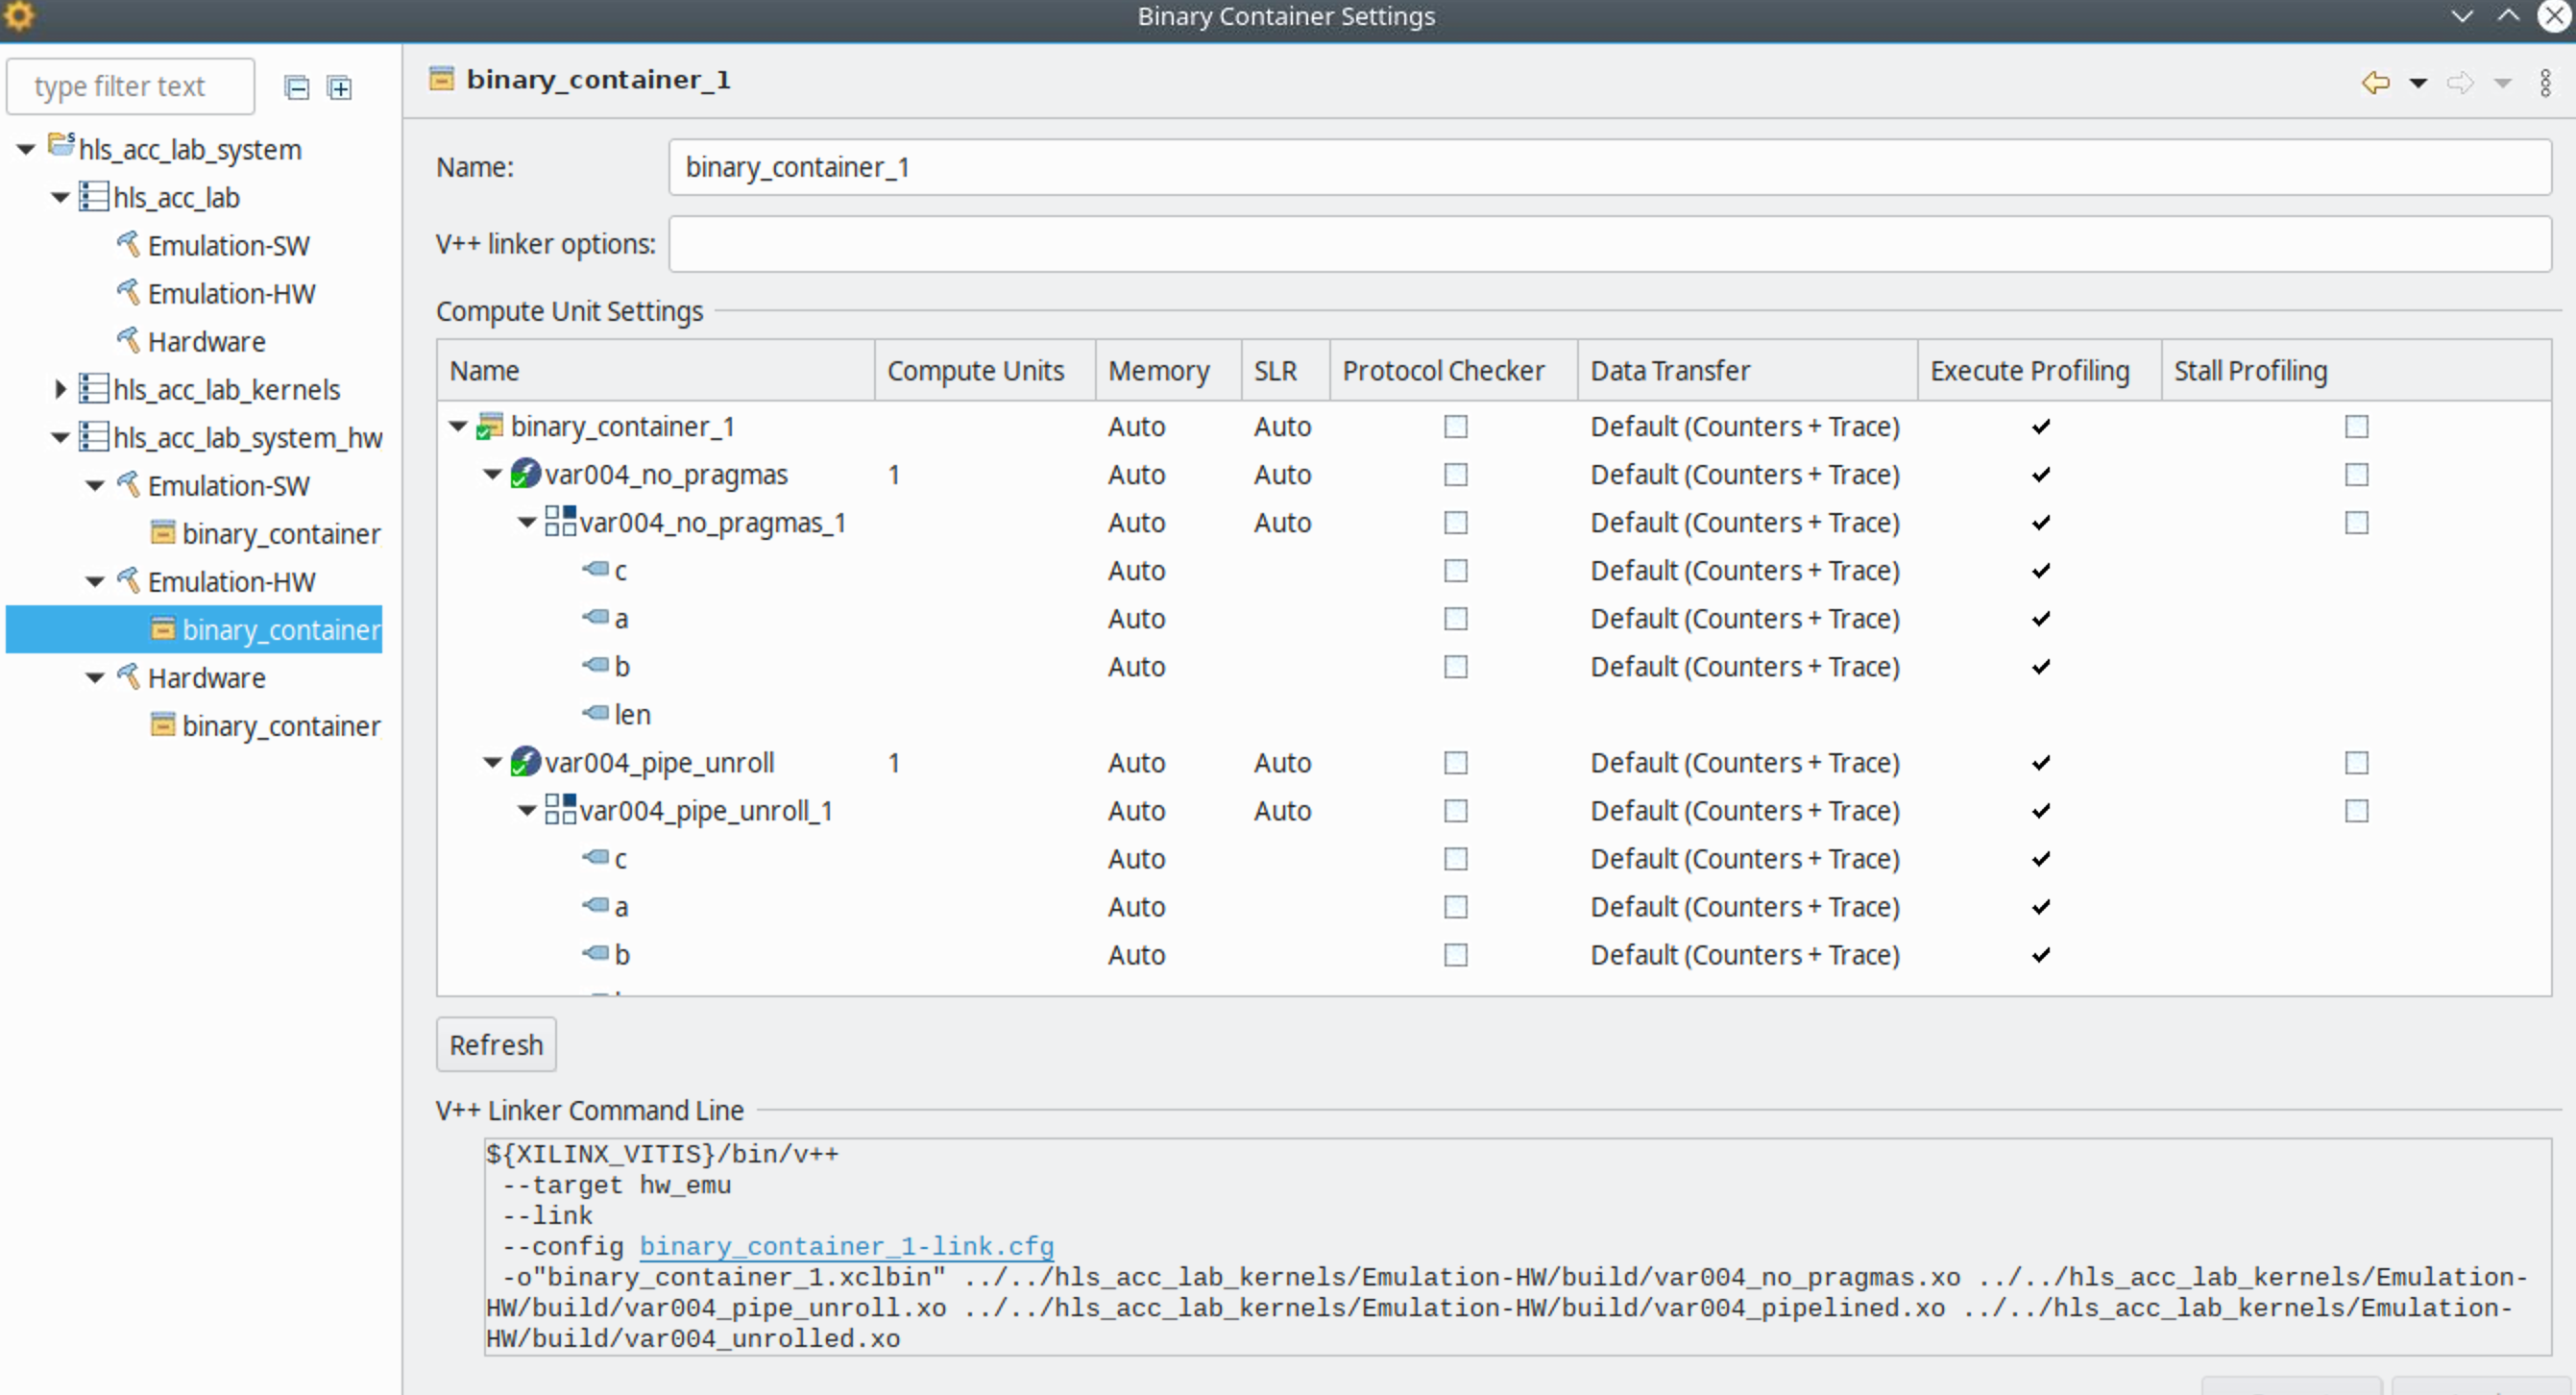
\includegraphics[width = \linewidth]{aview_1.png}
	\caption{Экран №1 Assistant View для сборки Emulation-HW}
	\label{img:aview_1}
\end{figure}

\begin{figure}[h!p]
	\centering
	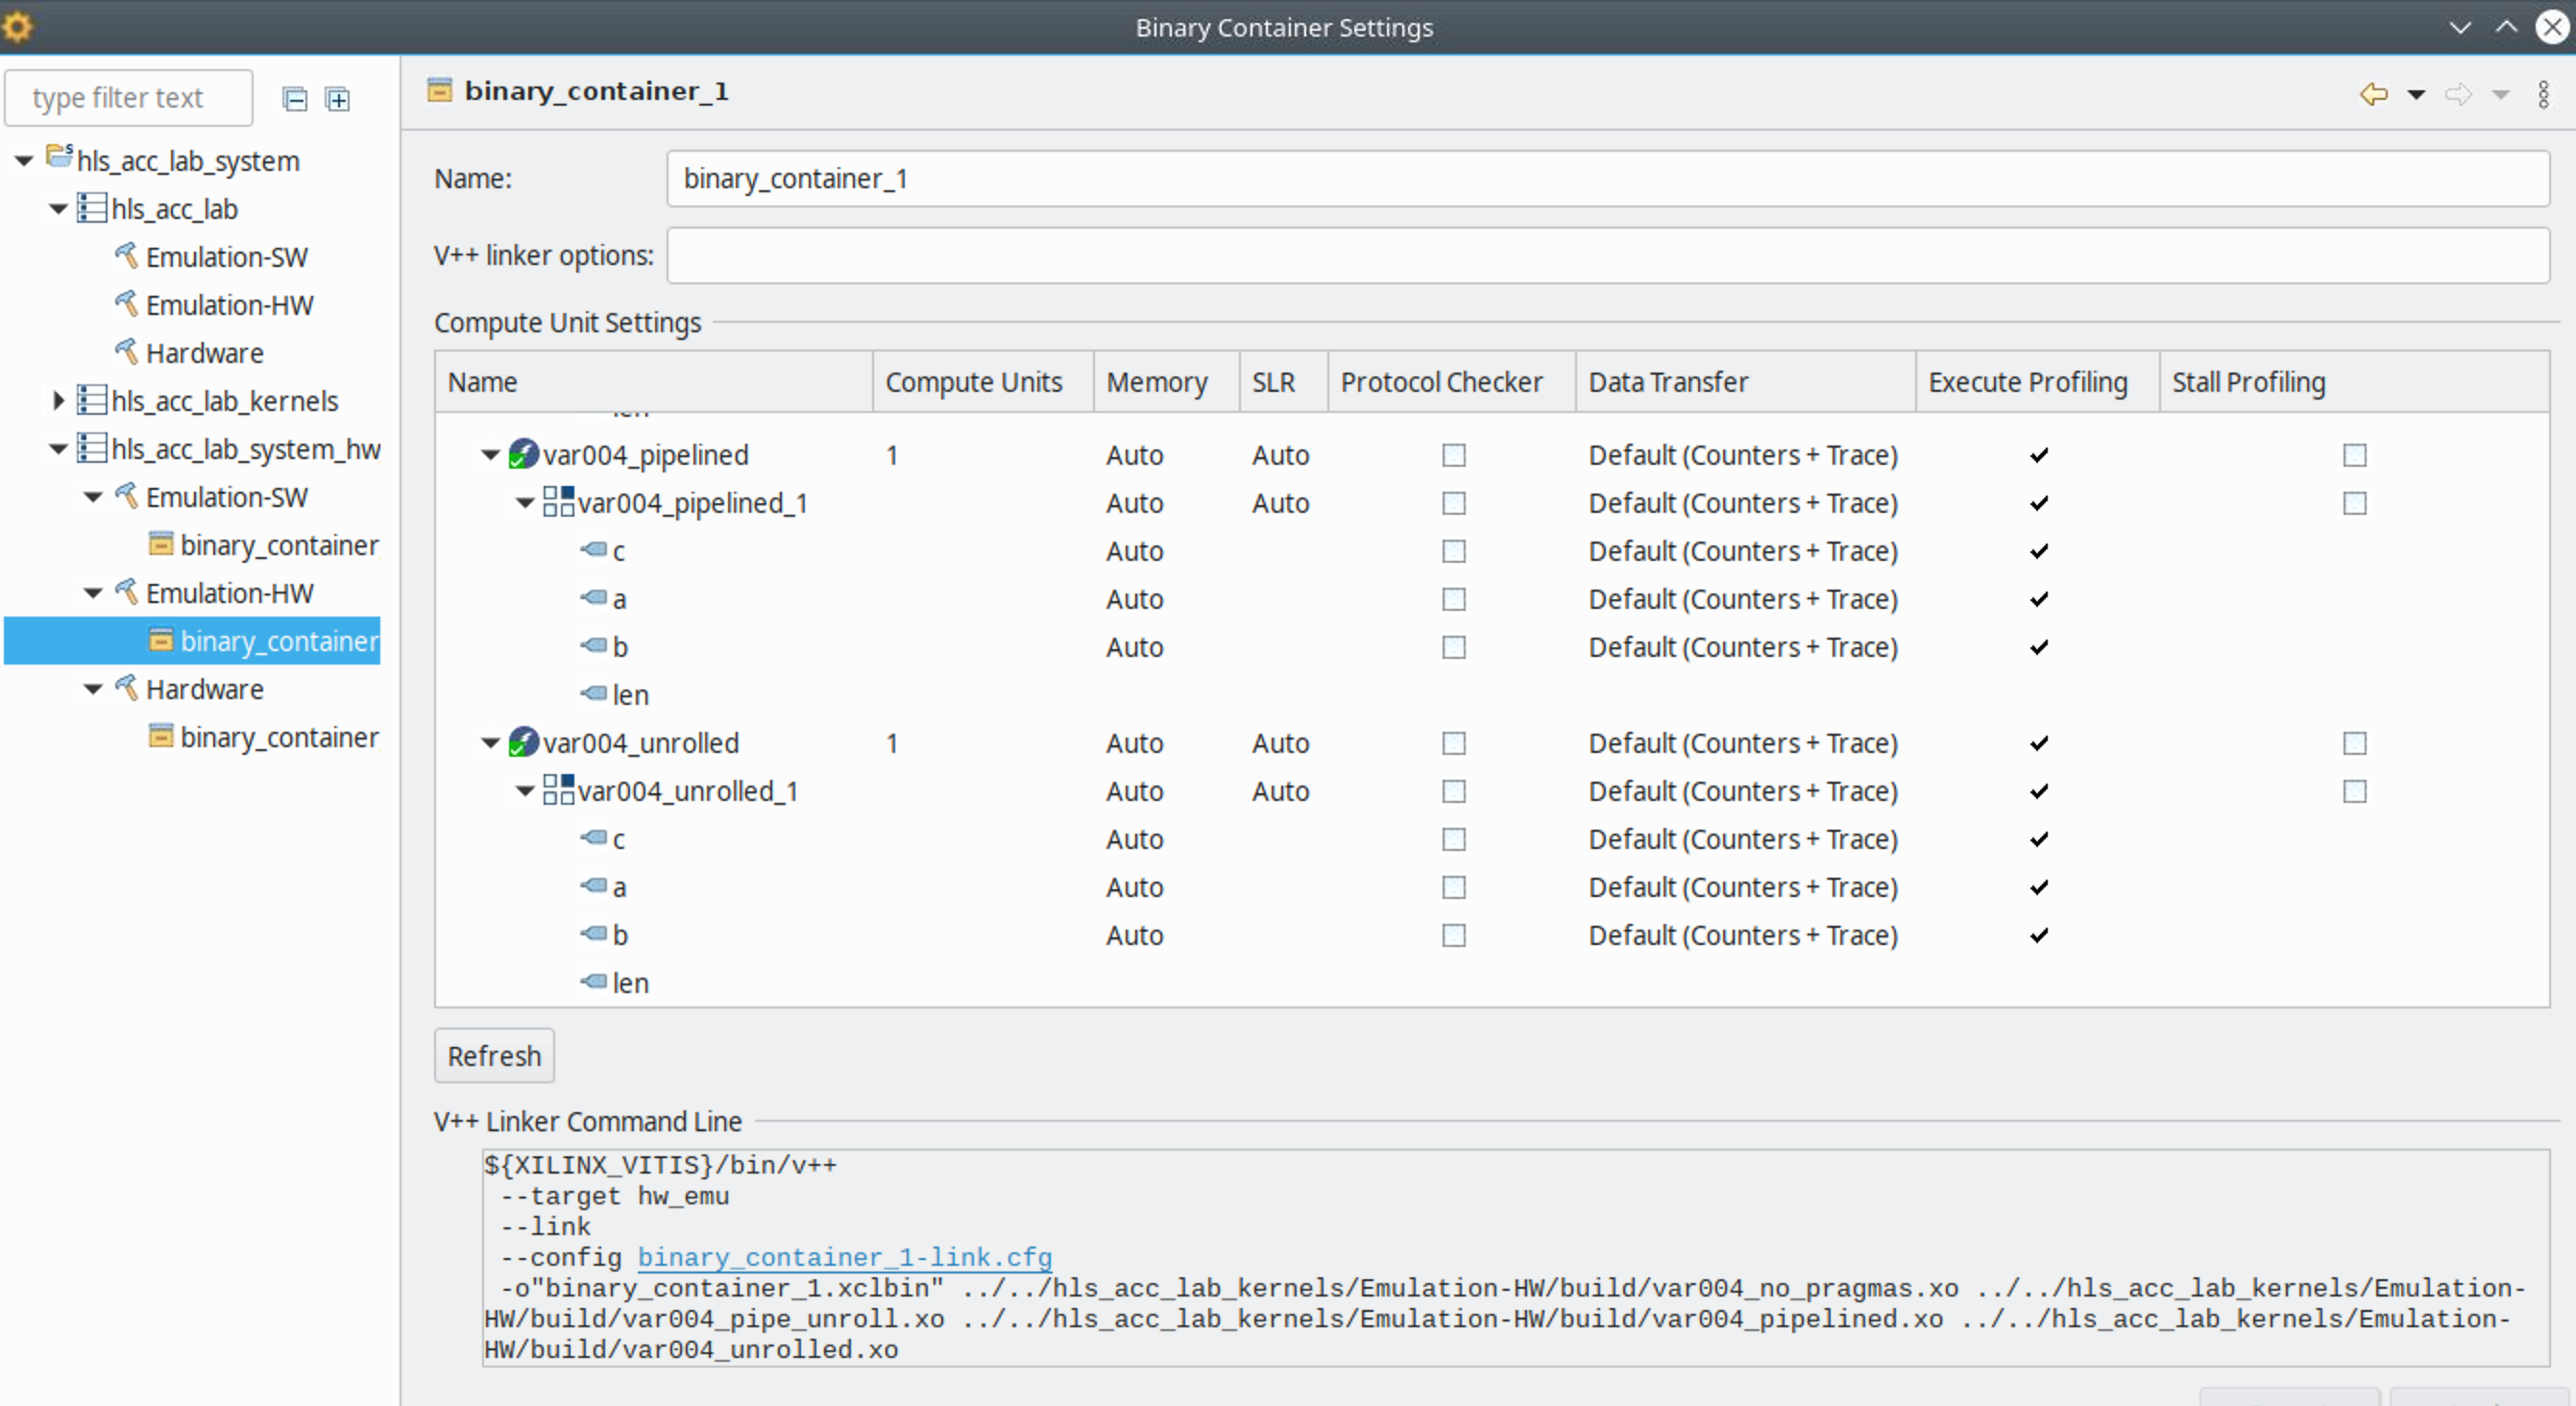
\includegraphics[width = \linewidth]{aview_2.png}
	\caption{Экран №2 Assistant View для сборки Emulation-HW}
	\label{img:aview_2}
\end{figure}

Результаты запуска приложения, которые были выданы на вкладку Console в режиме Emulation-HW приведены на рисунке \ref{img:test_hw_em}.
\begin{figure}[h!p]
	\centering
	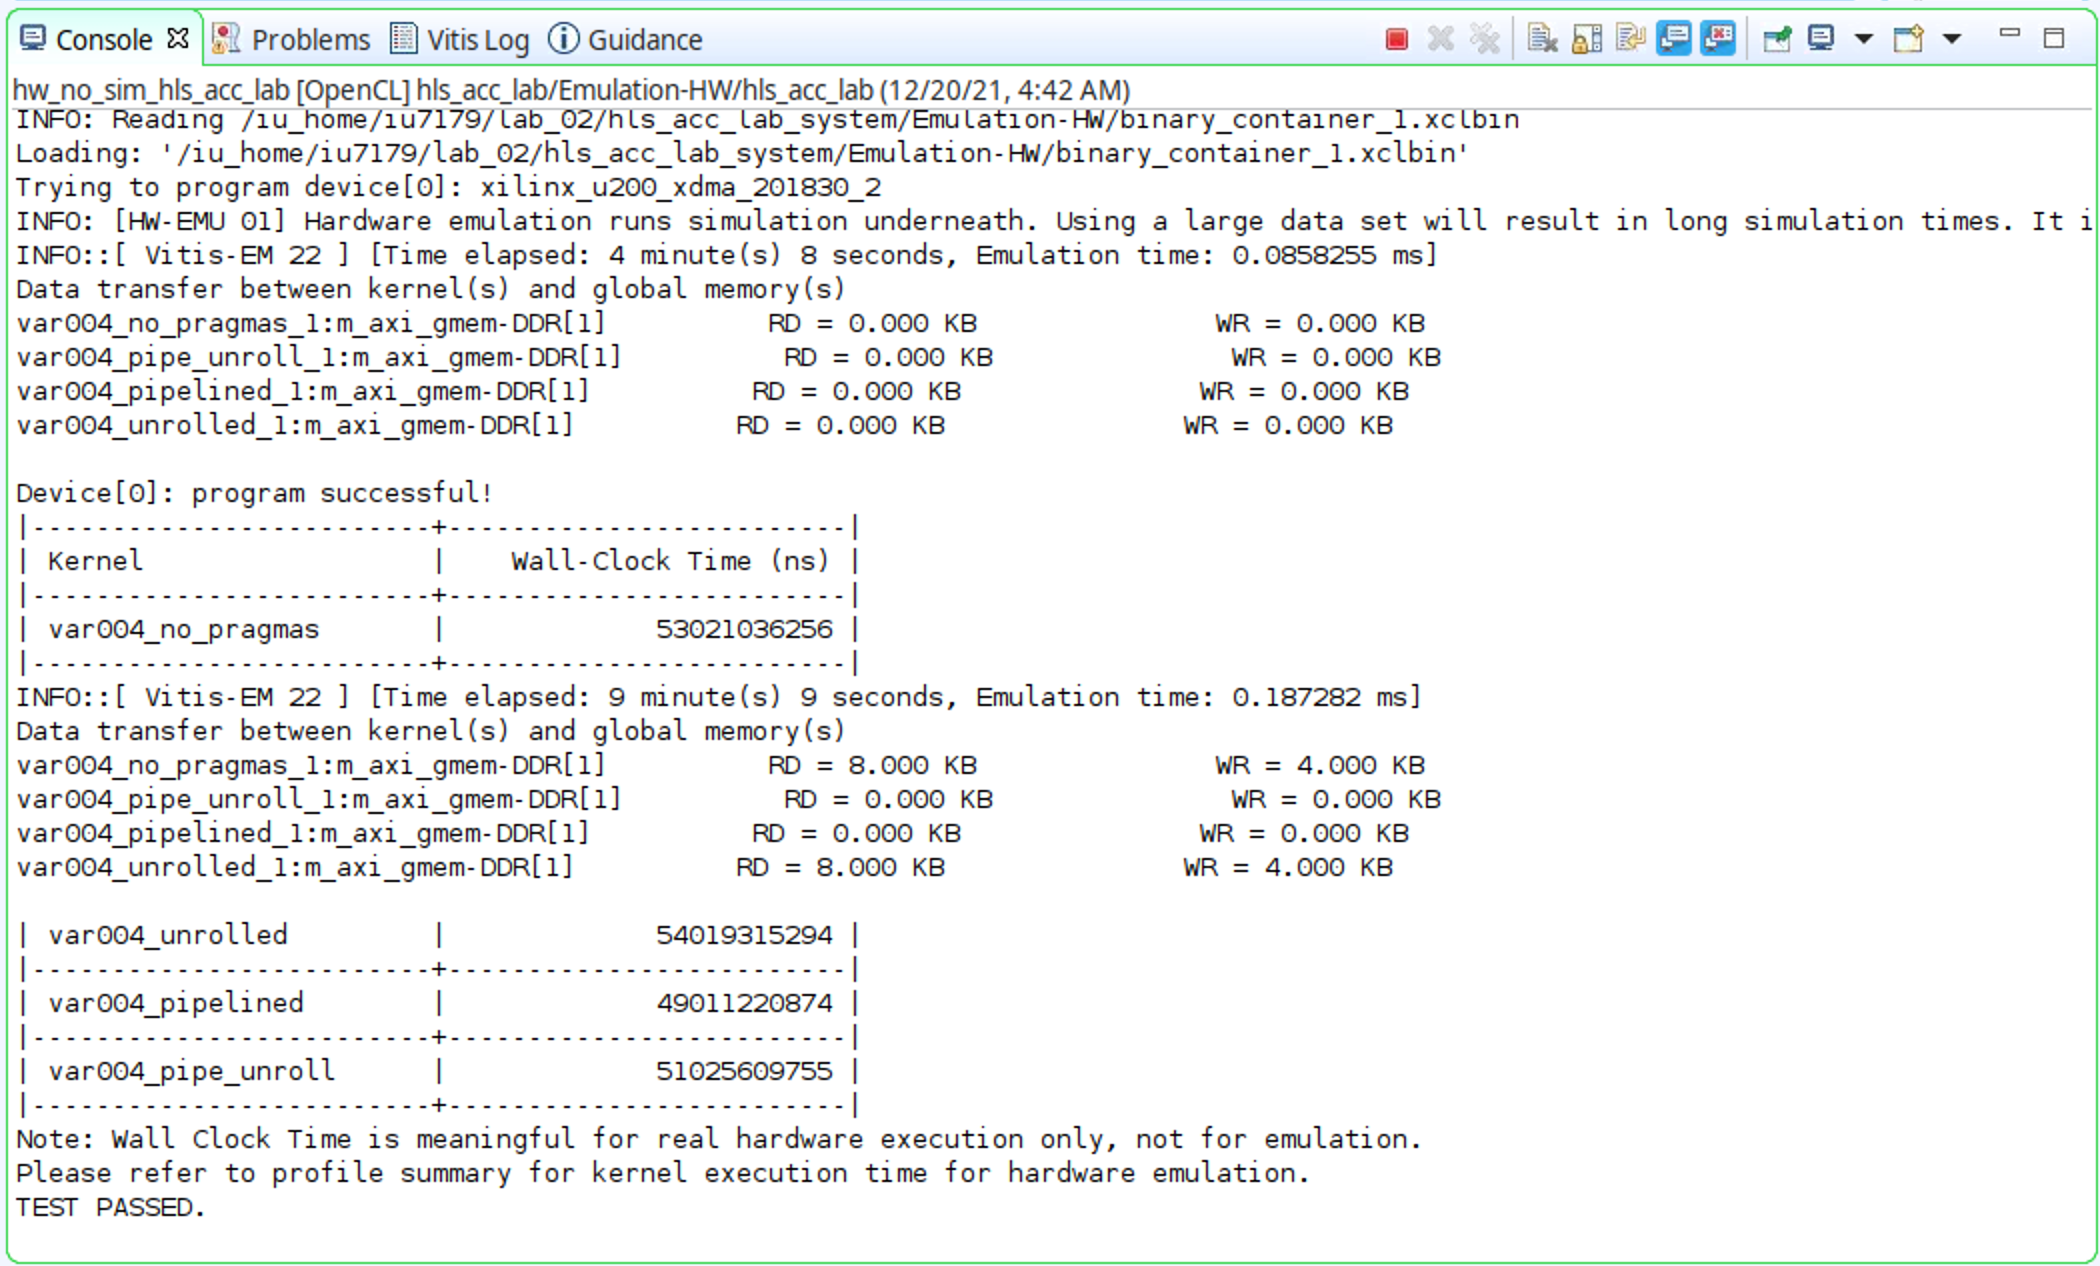
\includegraphics[width = \linewidth]{test_hw_em.png}
	\caption{Результаты запуска приложения в режиме Emulation-HW}
	\label{img:test_hw_em}
\end{figure}
\newpage
На рисунке \ref{img:dia} приведена диаграмма работы четырех ядер.
\begin{figure}[h!p]
	\centering
	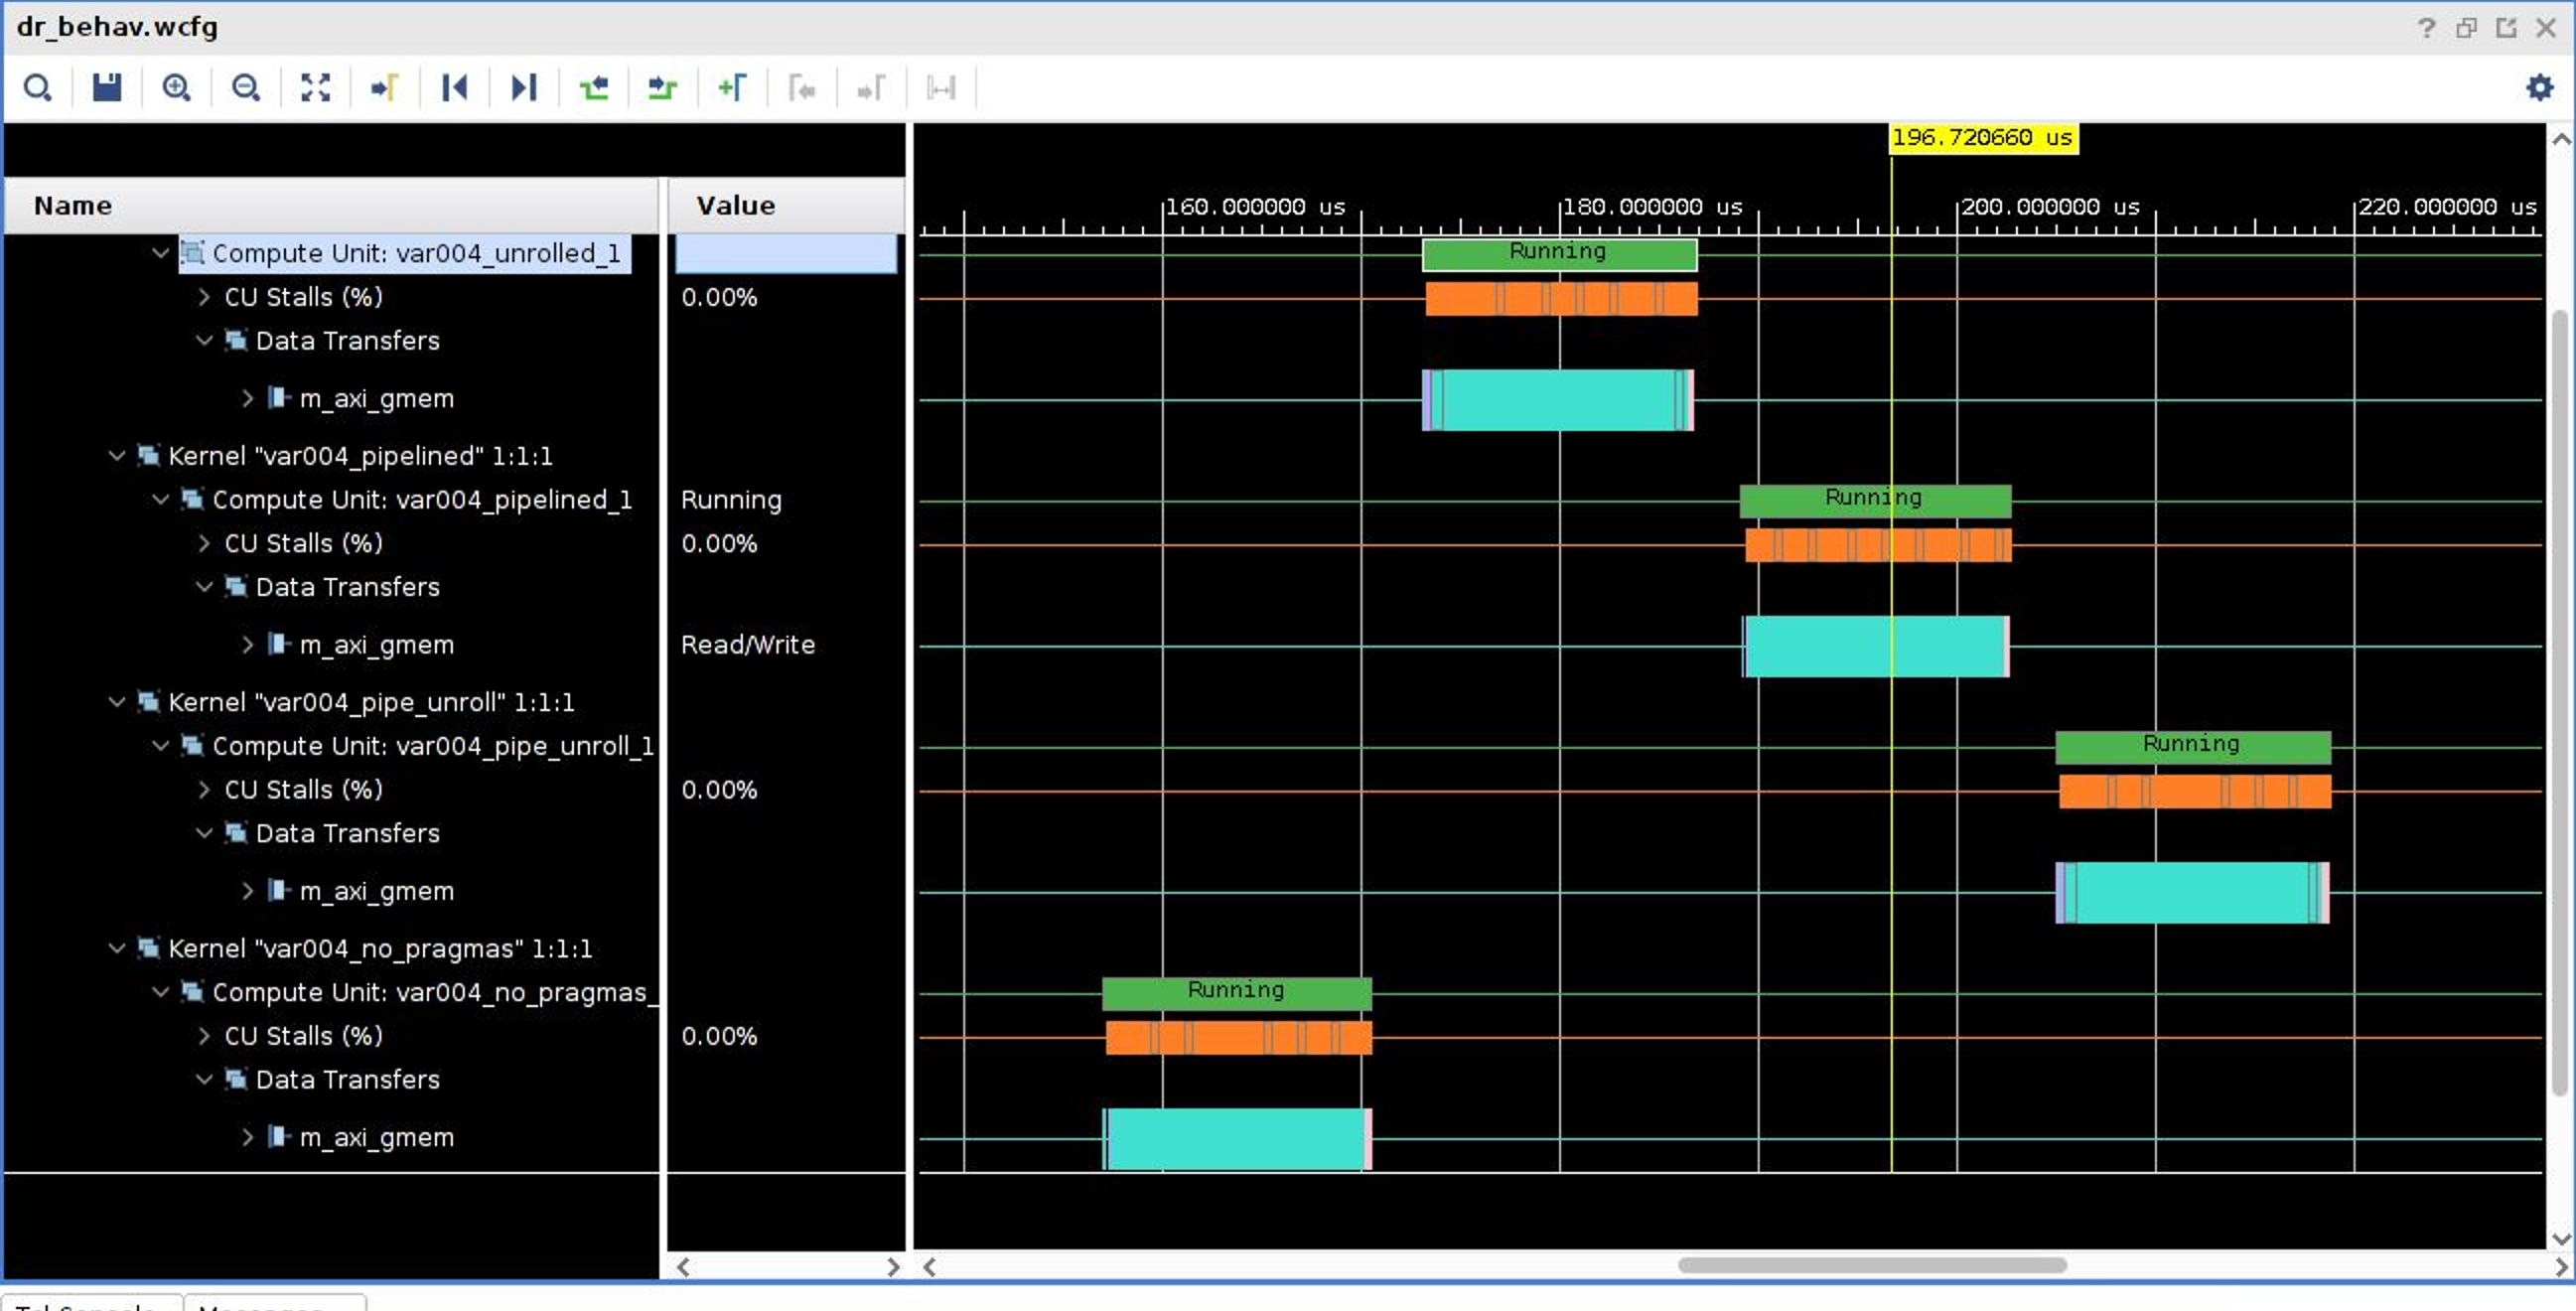
\includegraphics[width = \linewidth]{dia.png}
	\caption{Диаграмма работы четырех ядер}
	\label{img:dia}
\end{figure}

\chapter{Сборка и отладка проекта в режиме аппаратного исполнения (Hardware)}
Результаты запуска приложения, которые были выданы на вкладку Console в режиме Hardware приведены на рисунке \ref{img:test_hw}.

\begin{figure}[h!p]
	\centering
	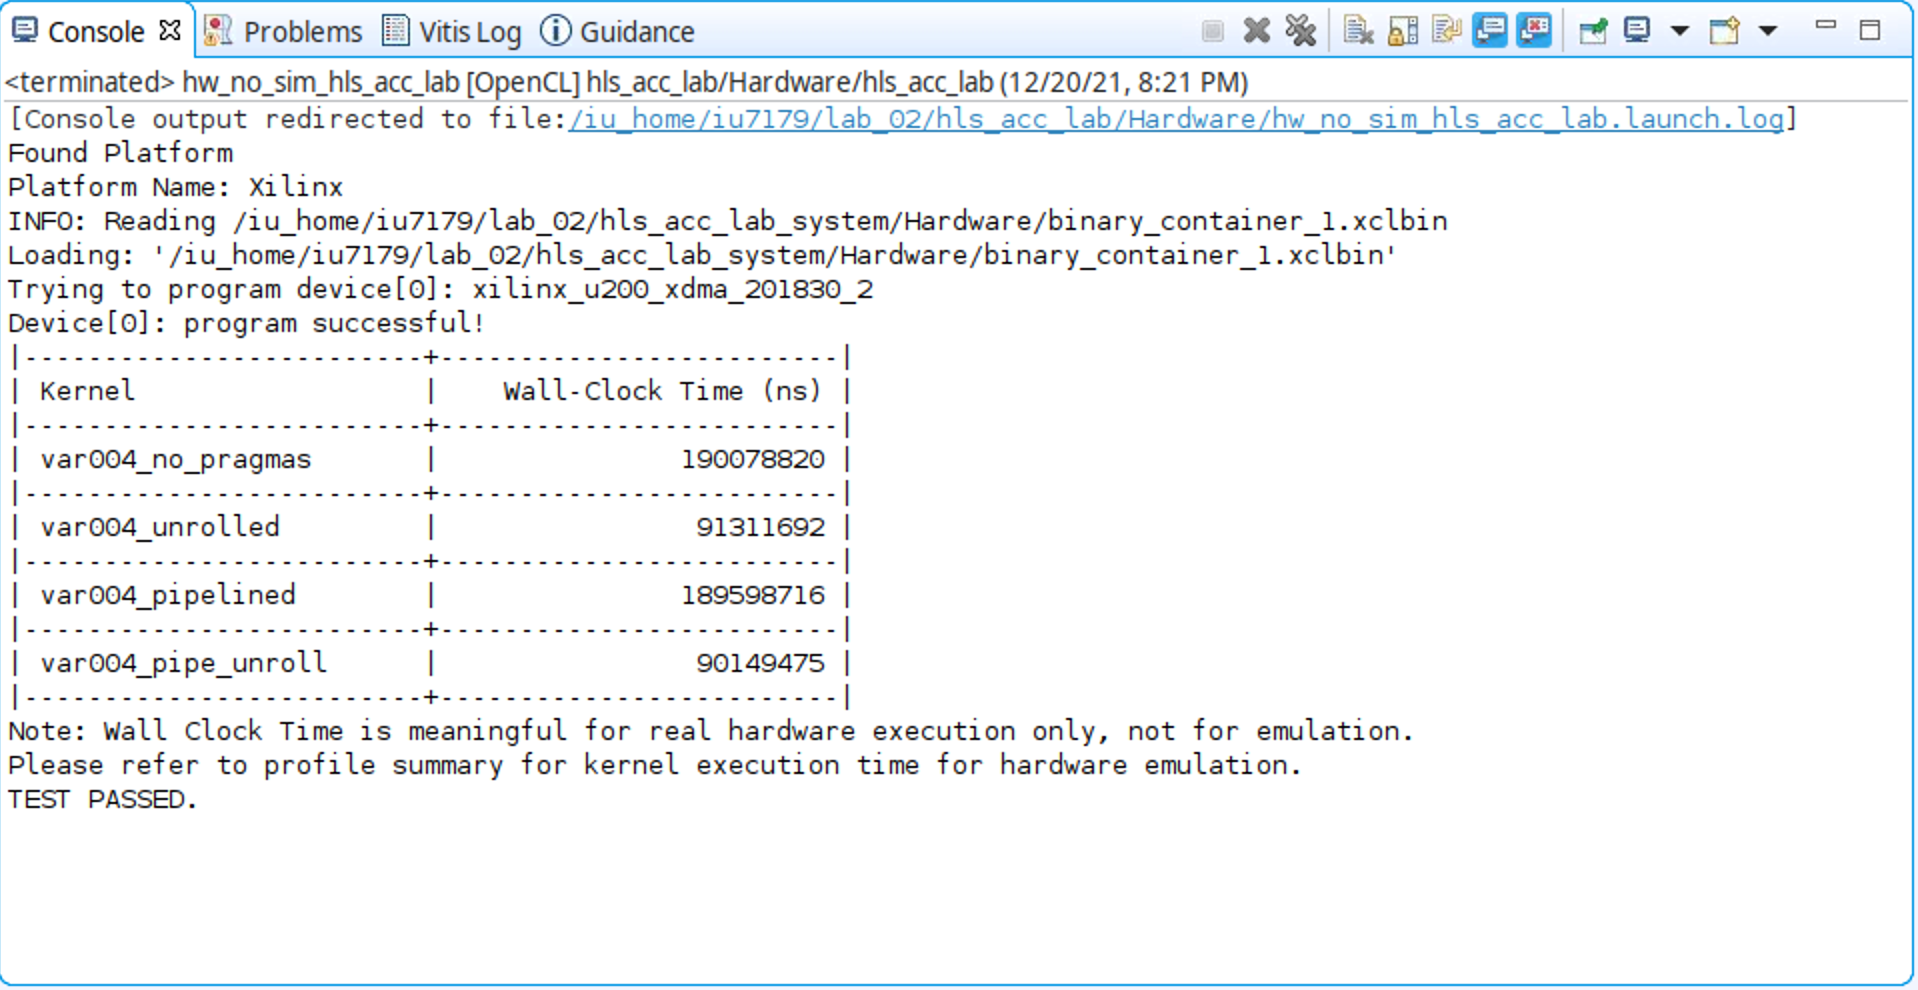
\includegraphics[width = \linewidth]{test_hw.png}
	\caption{Результаты запуска приложения в режиме Hardware}
	\label{img:test_hw}
\end{figure}
\newpage
Копии экранов для вкладок «Summary», «System Diagram», «Platform Diagram» и четрые вкладки «HLS Synthesis» для каждого ядра приведены на рисунках \ref{img:sum} - \ref{img:syn_pipe_unroll}.

\begin{figure}[h!p]
	\centering
	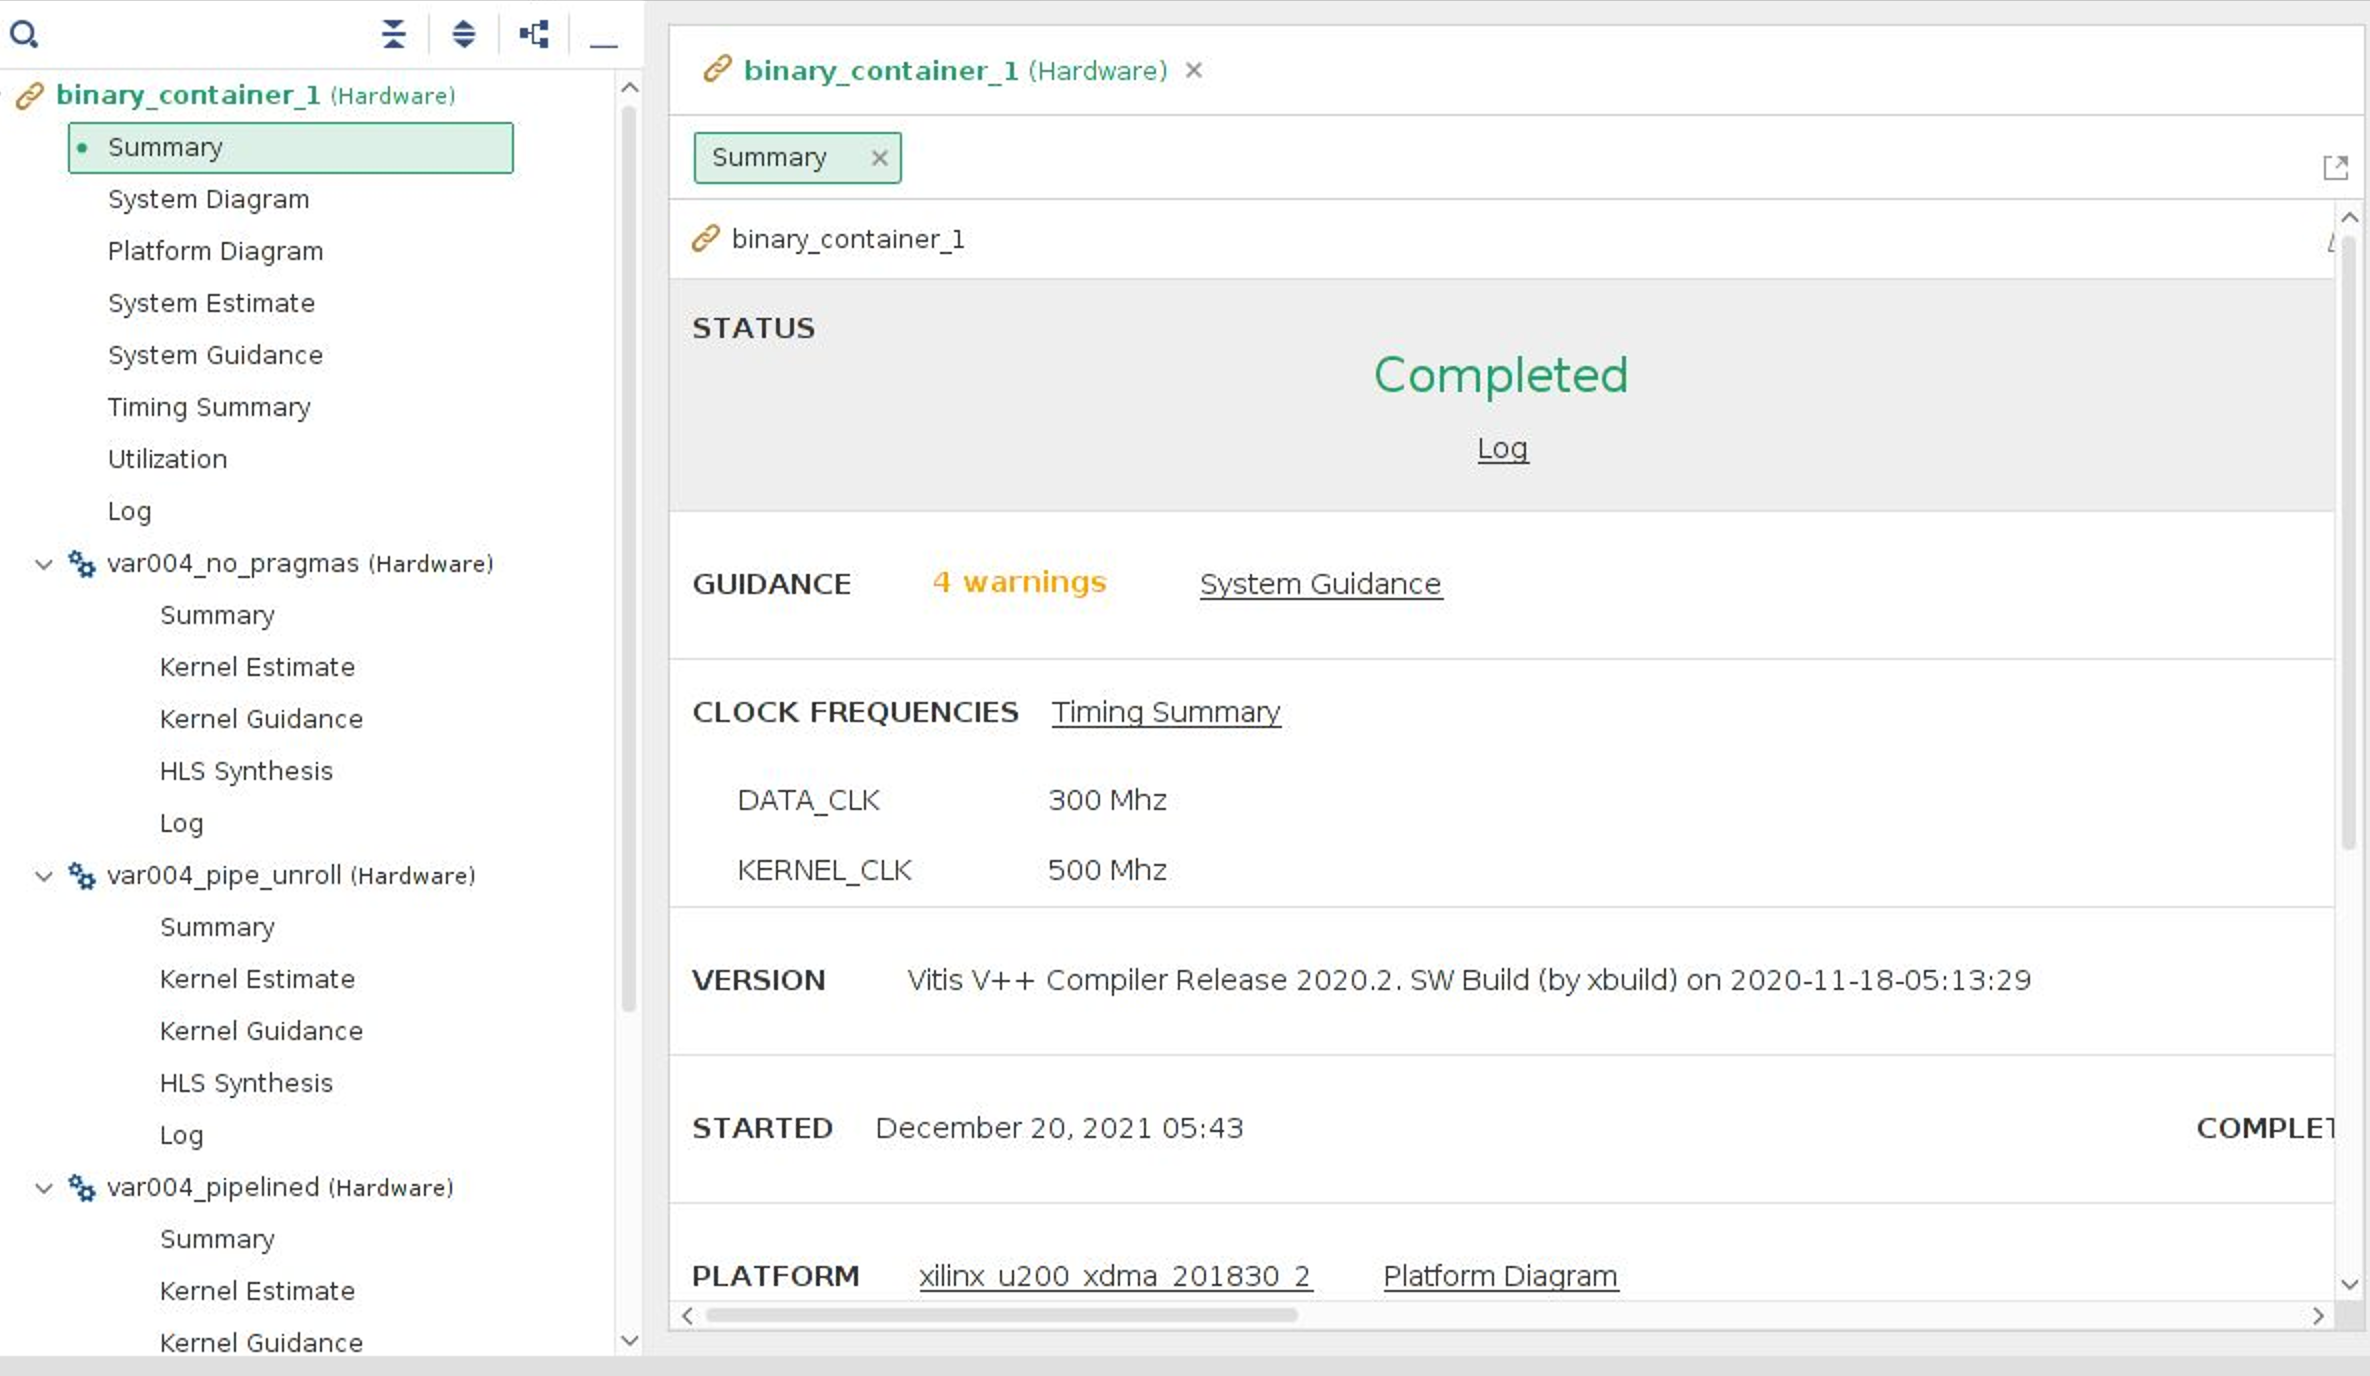
\includegraphics[scale = 0.37]{sum.png}
	\caption{Копия экрана для вкладки «Summary»}
	\label{img:sum}
\end{figure}
\begin{figure}[h!p]
	\centering
	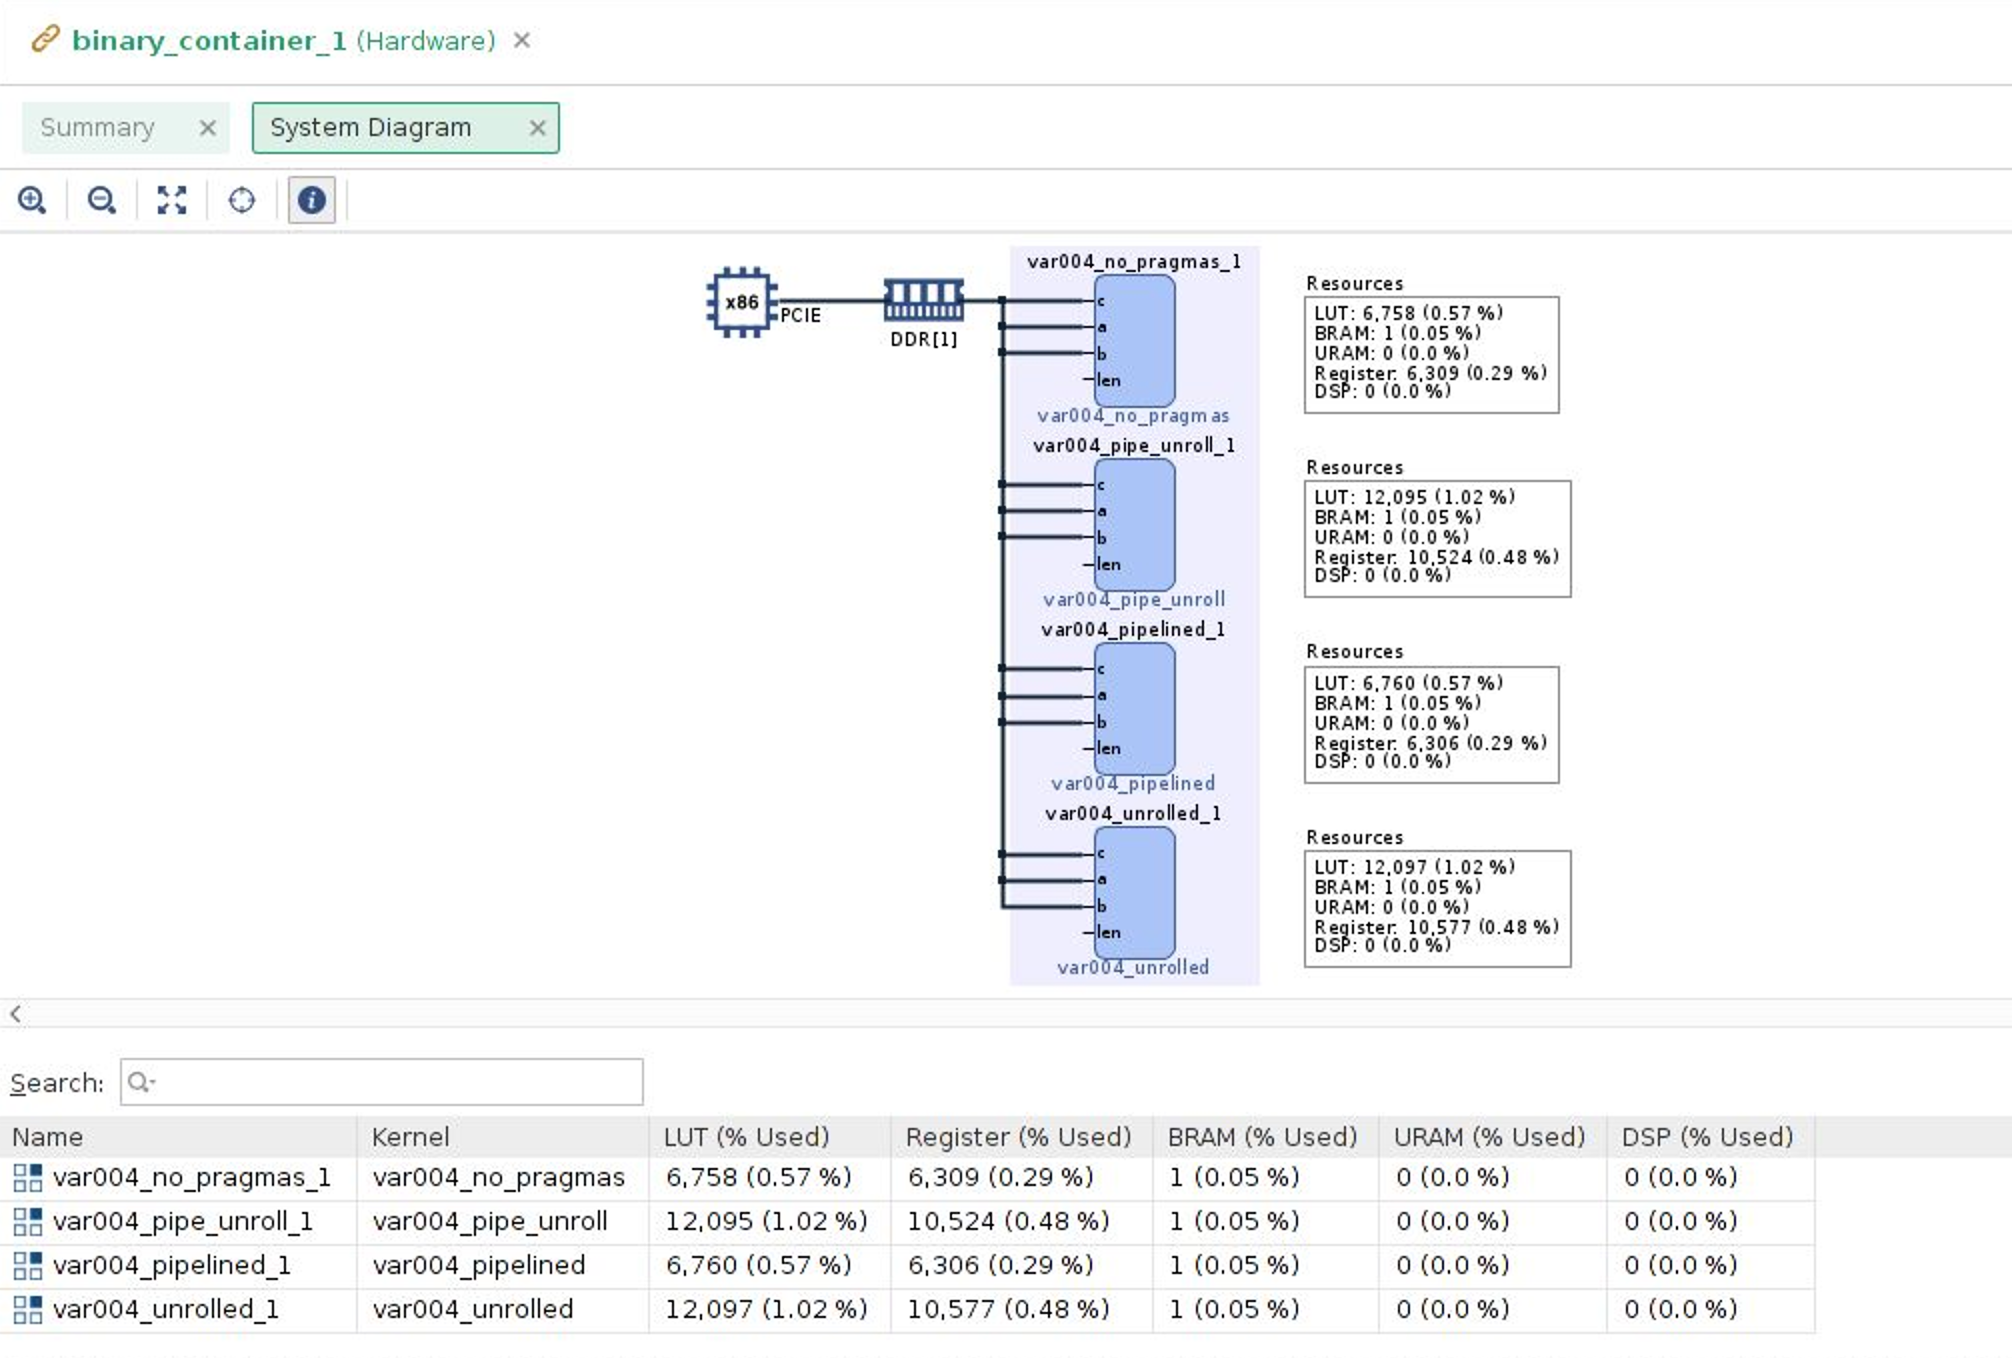
\includegraphics[scale = 0.42]{sys_dia.png}
	\caption{Копия экрана для вкладки «System Diagram»}
	\label{img:sys_dia}
\end{figure}
\begin{figure}[h!p]
	\centering
	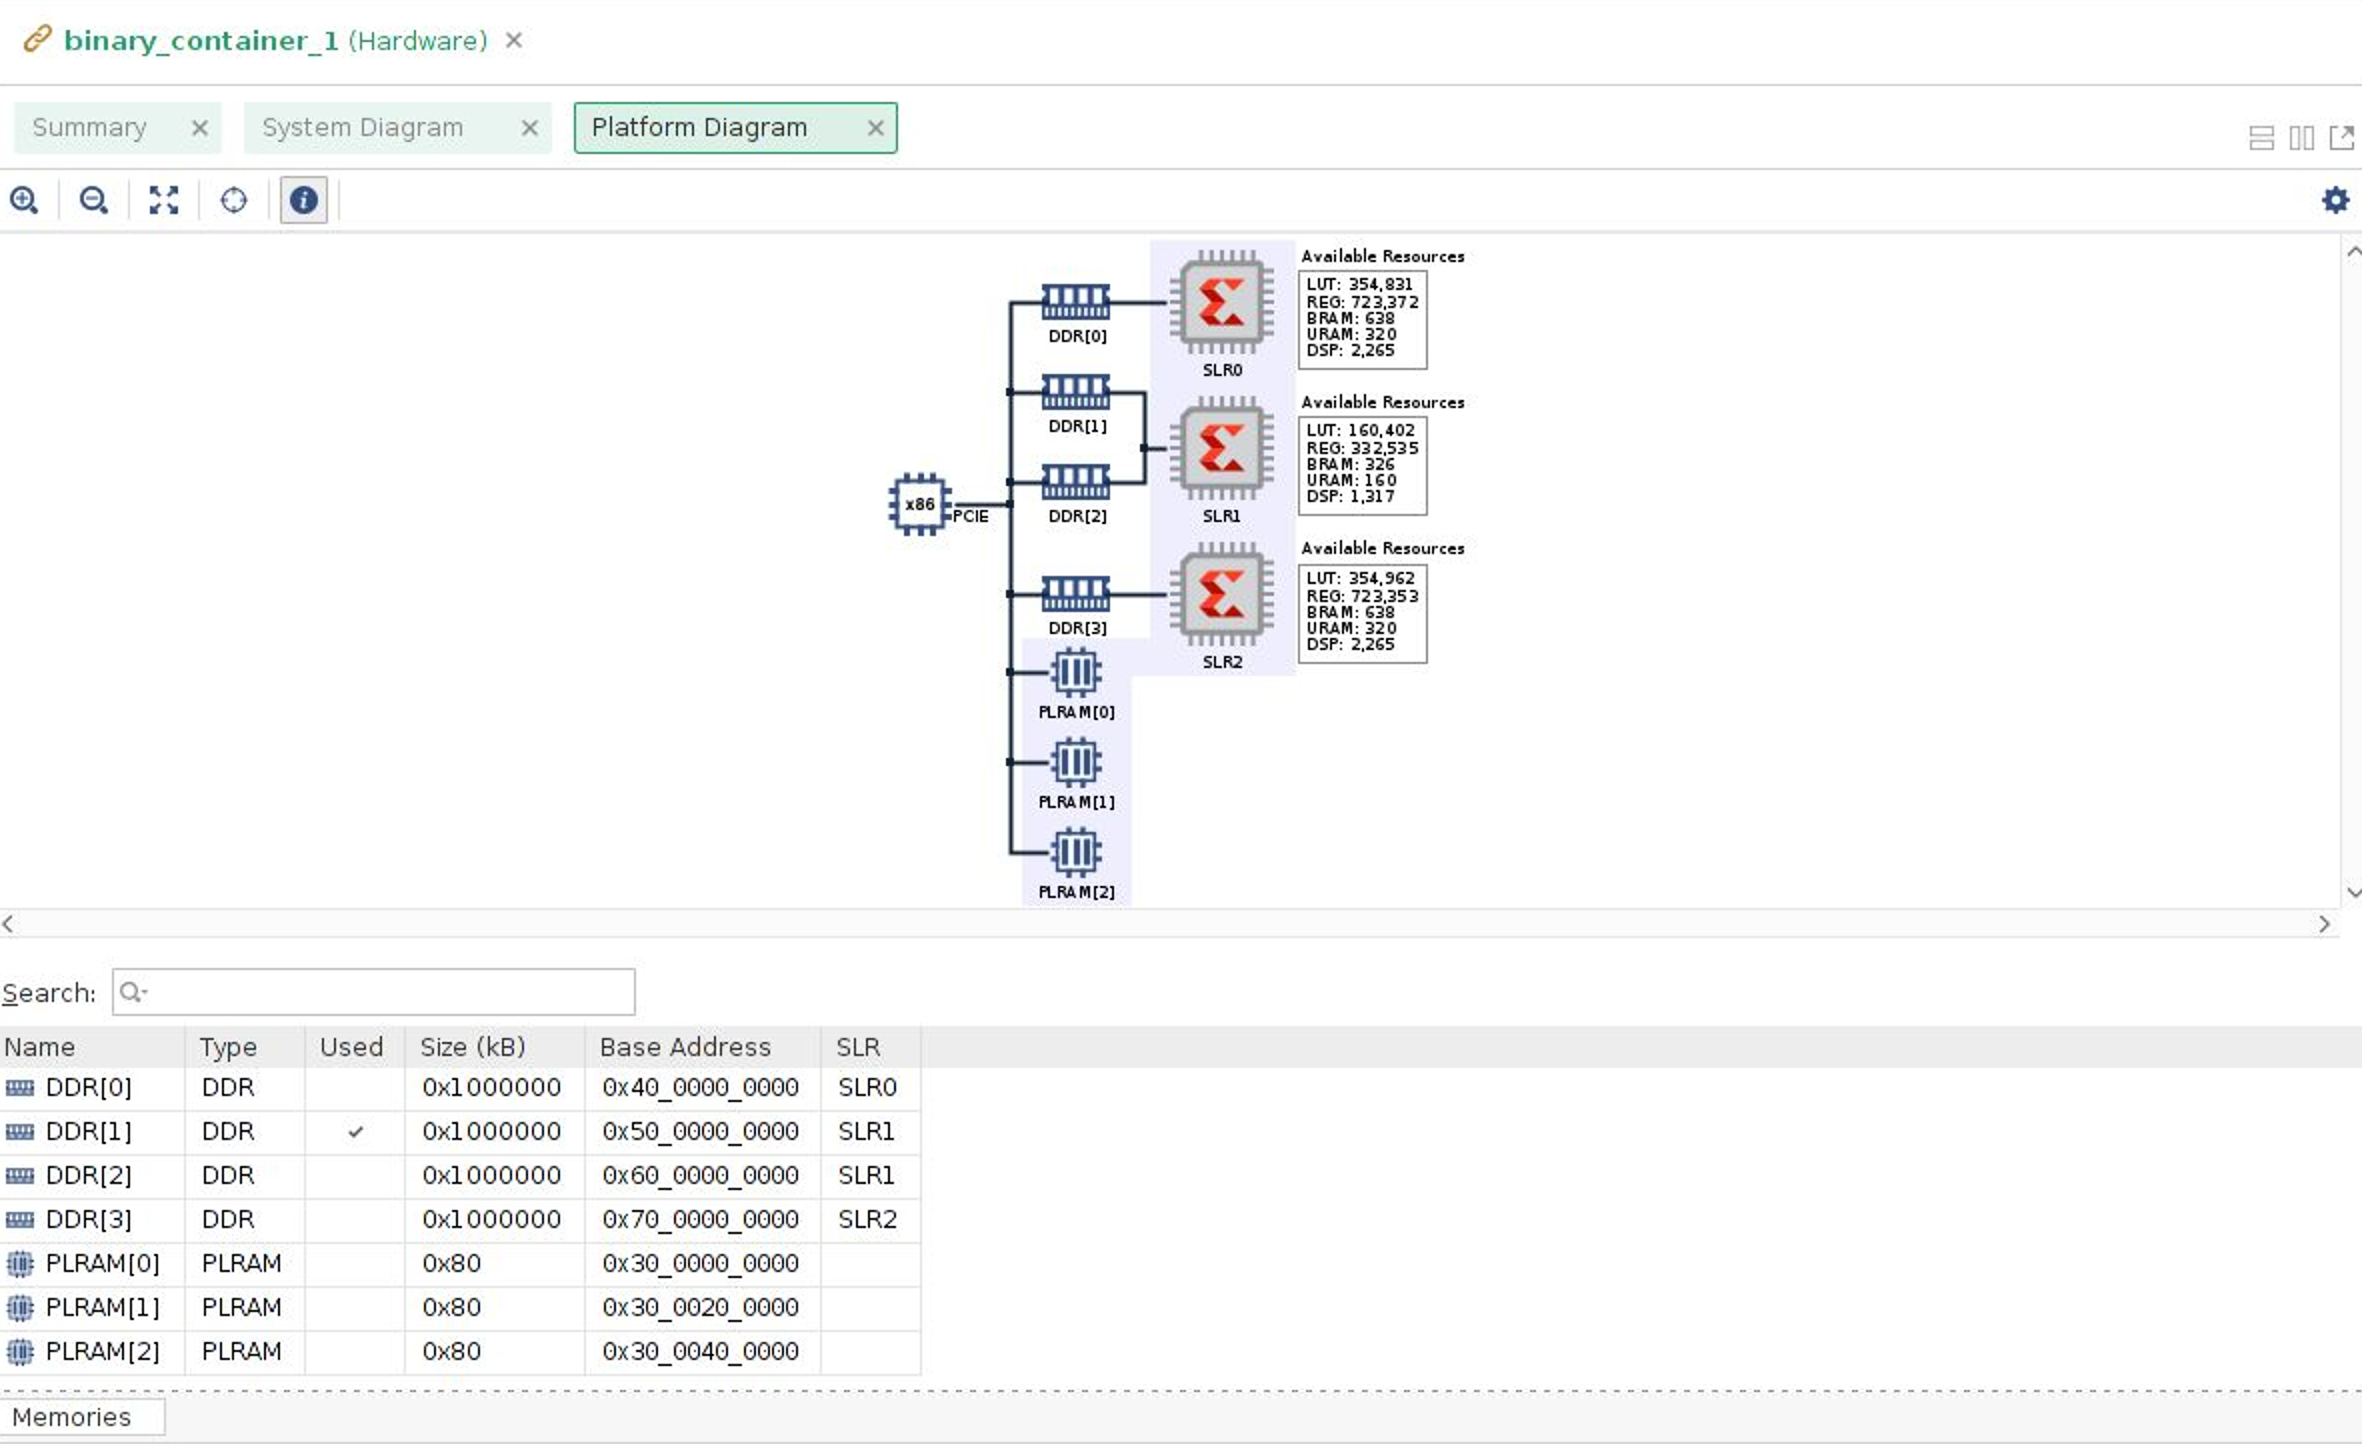
\includegraphics[width = \linewidth]{plat_dia.png}
	\caption{Копия экрана для вкладки «Platform Diagram»}
	\label{img:plat_dia}
\end{figure}
\begin{figure}[h!p]
	\centering
	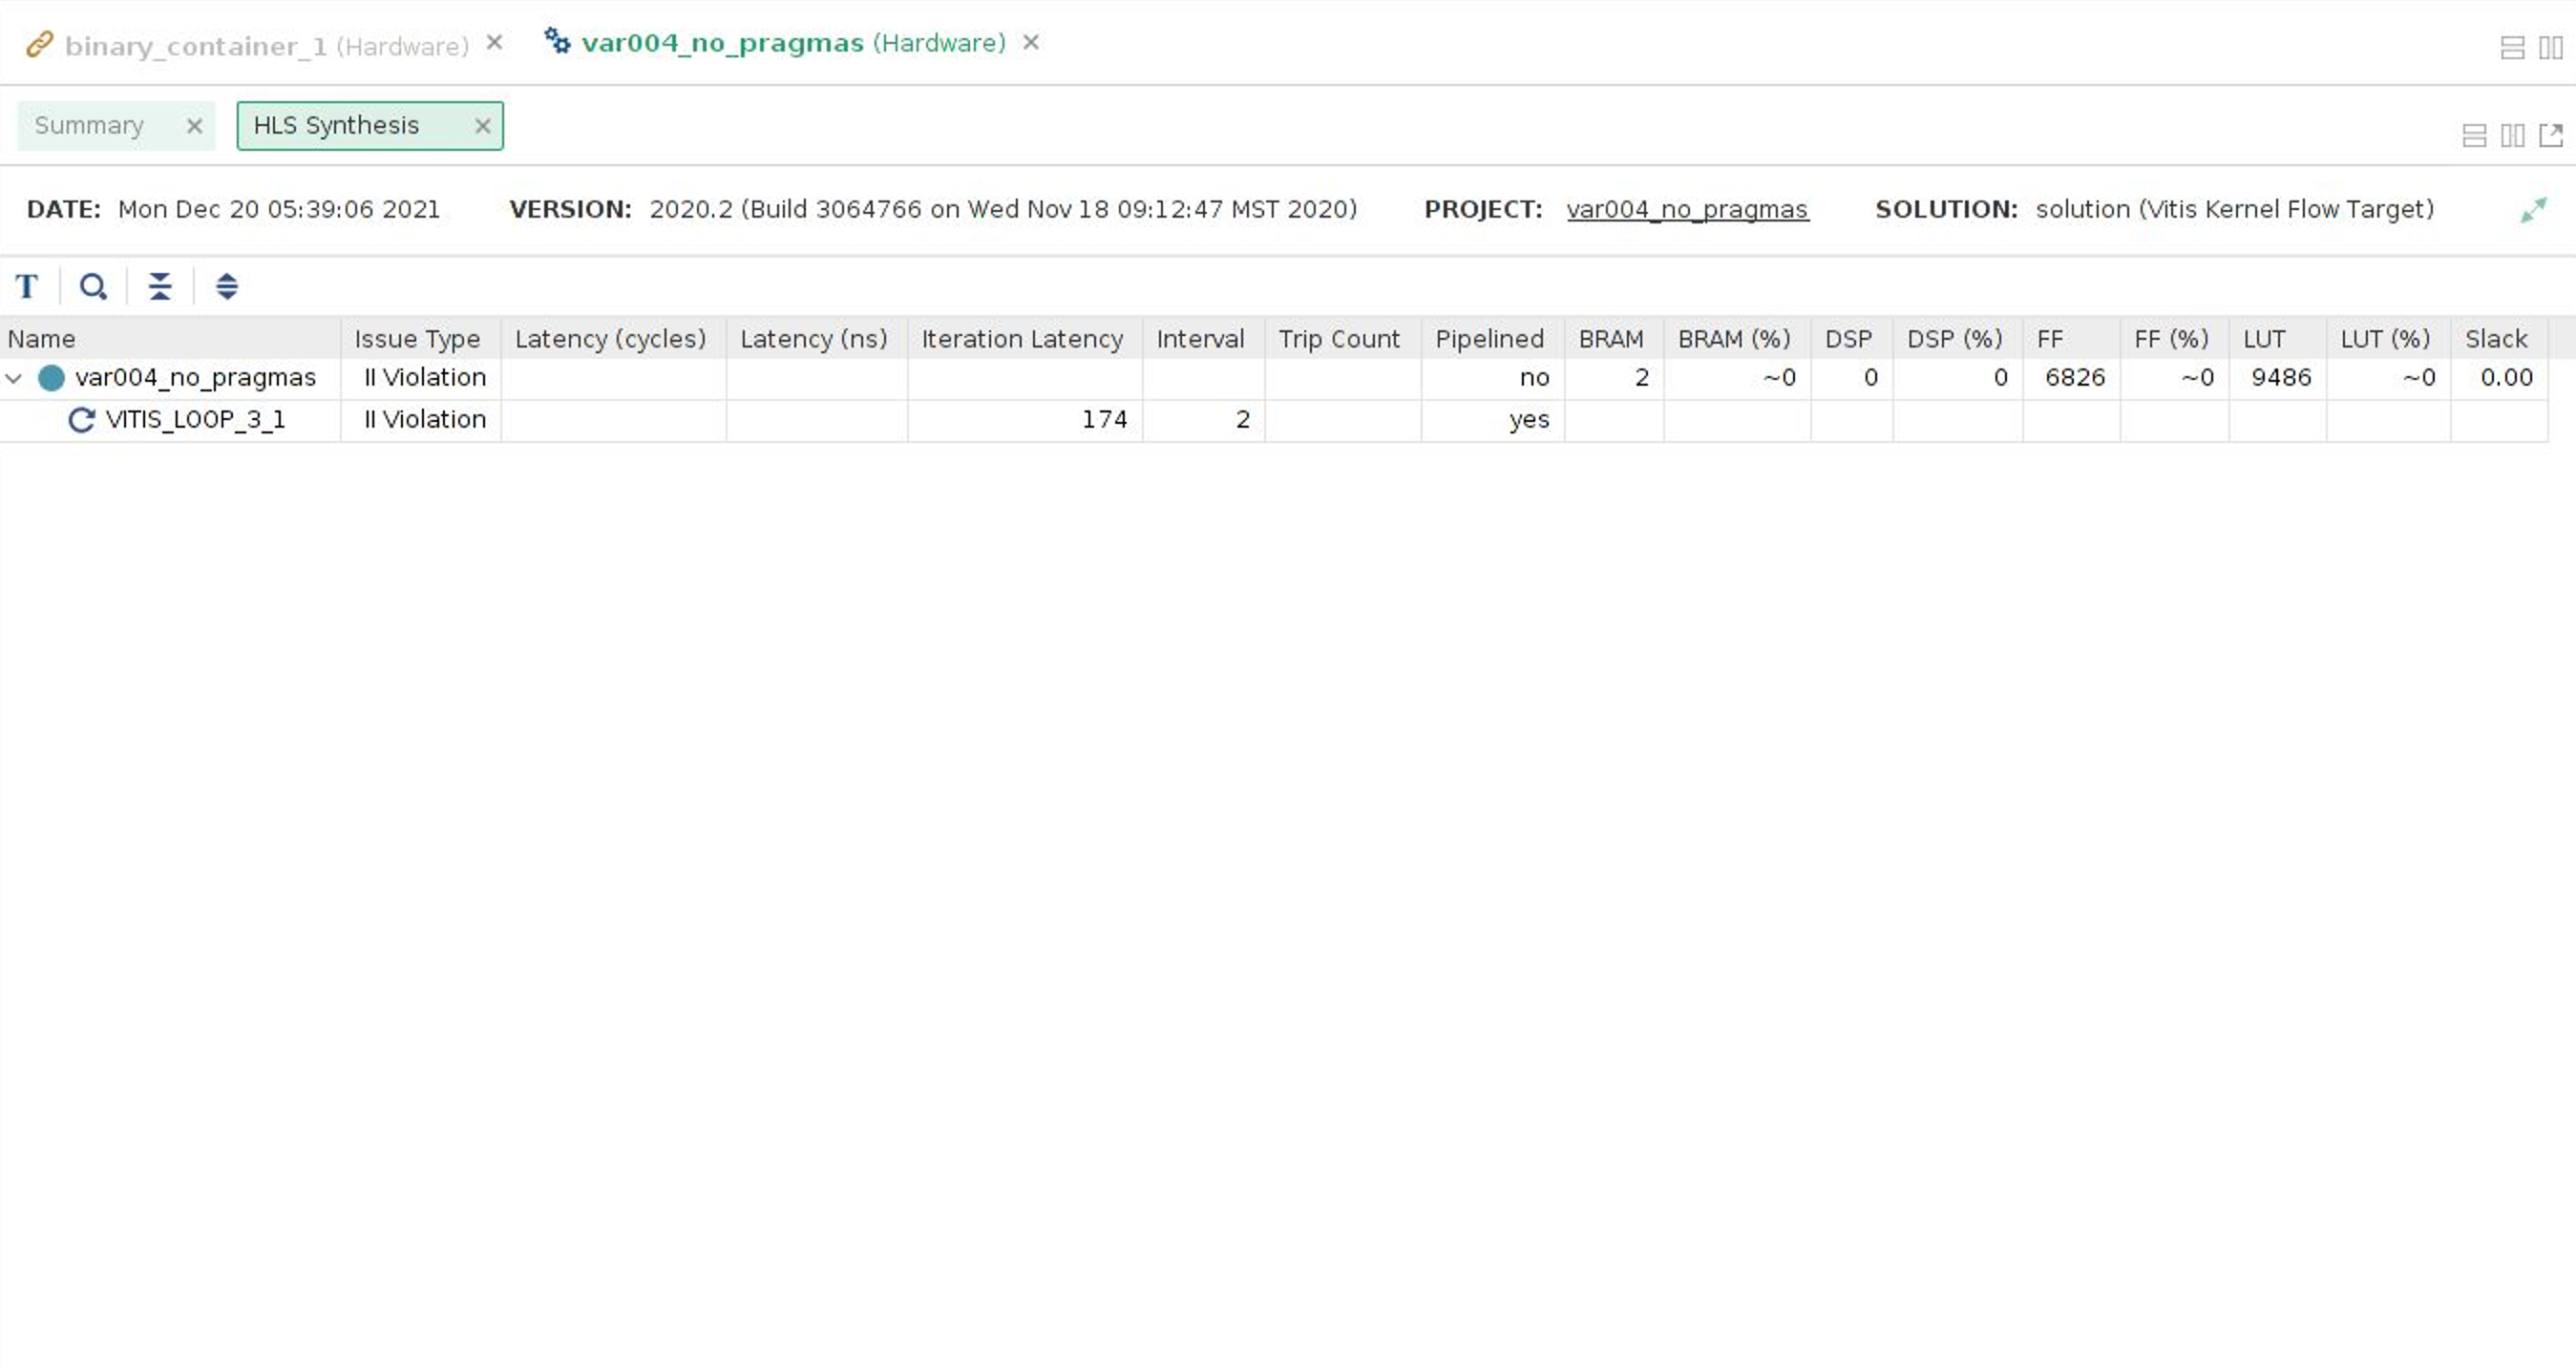
\includegraphics[width = \linewidth]{syn_no_pragmas.png}
	\caption{Копия экрана для вкладки «HLS Synthesis» для ядра без оптимизации цикла}
	\label{img:syn_no_pragmas}
\end{figure}
\begin{figure}[h!p]
	\centering
	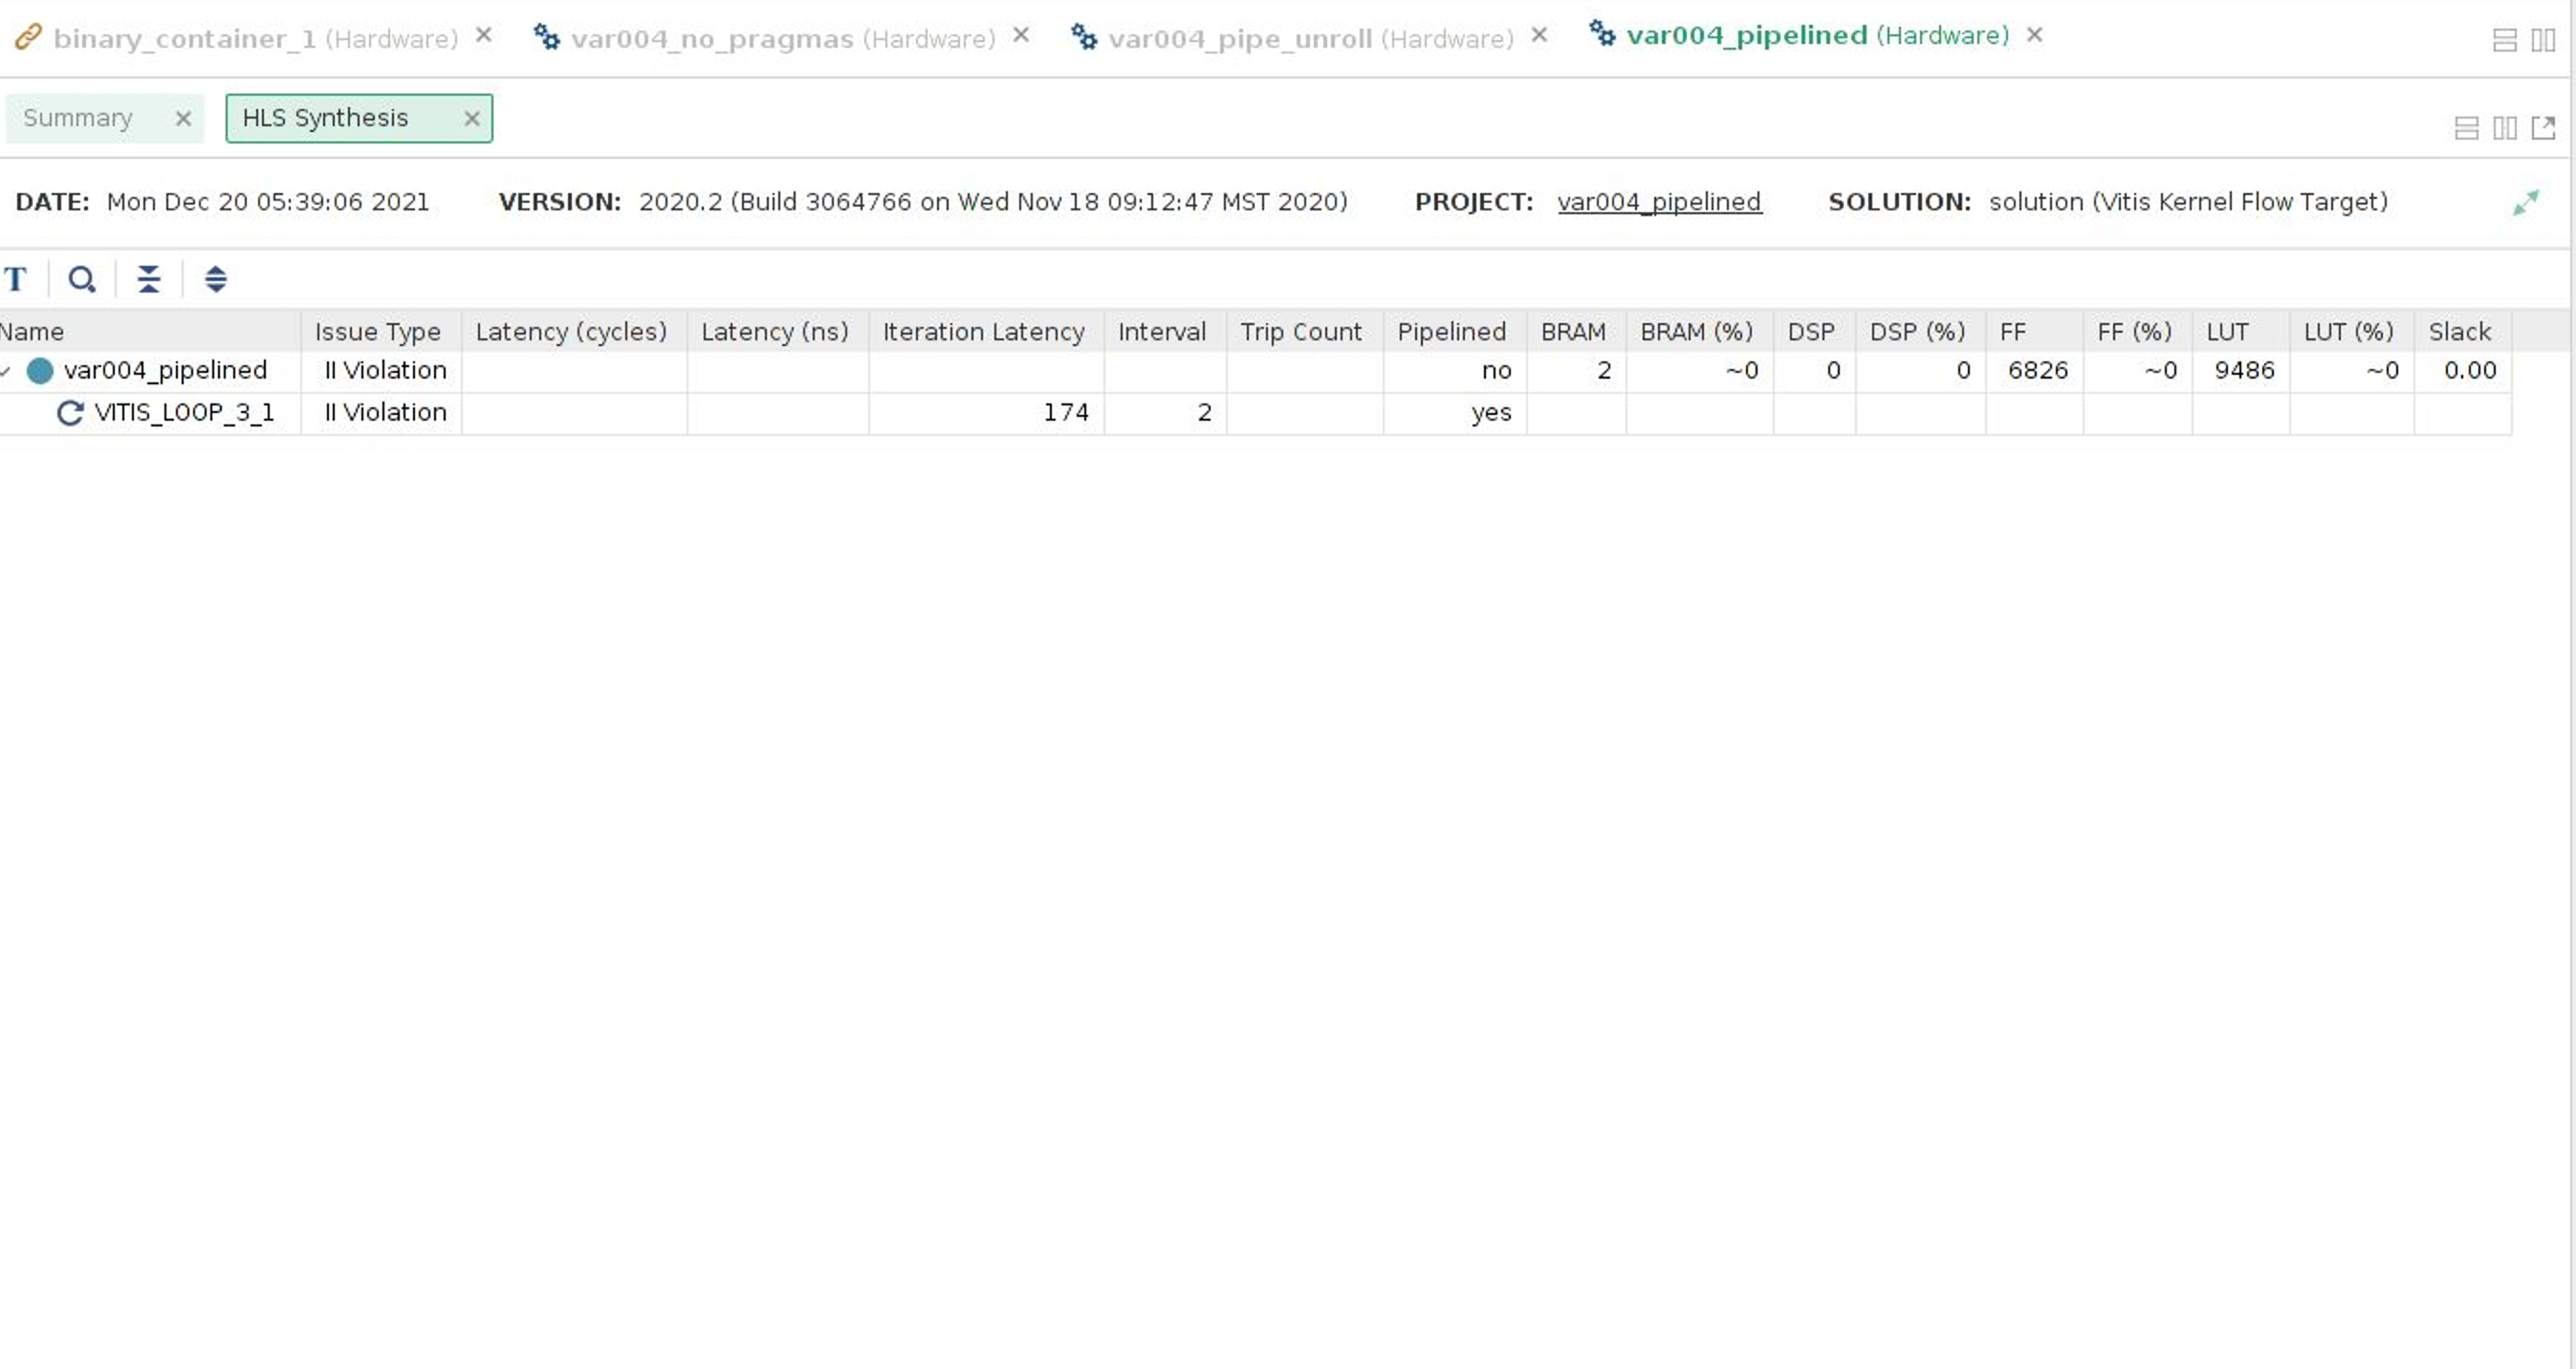
\includegraphics[width = \linewidth]{syn_pipelined.png}
	\caption{Копия экрана для вкладки «HLS Synthesis» для ядра с конвейерной организацией цикла}
	\label{img:syn_pipelined}
\end{figure}
\begin{figure}[h!p]
	\centering
	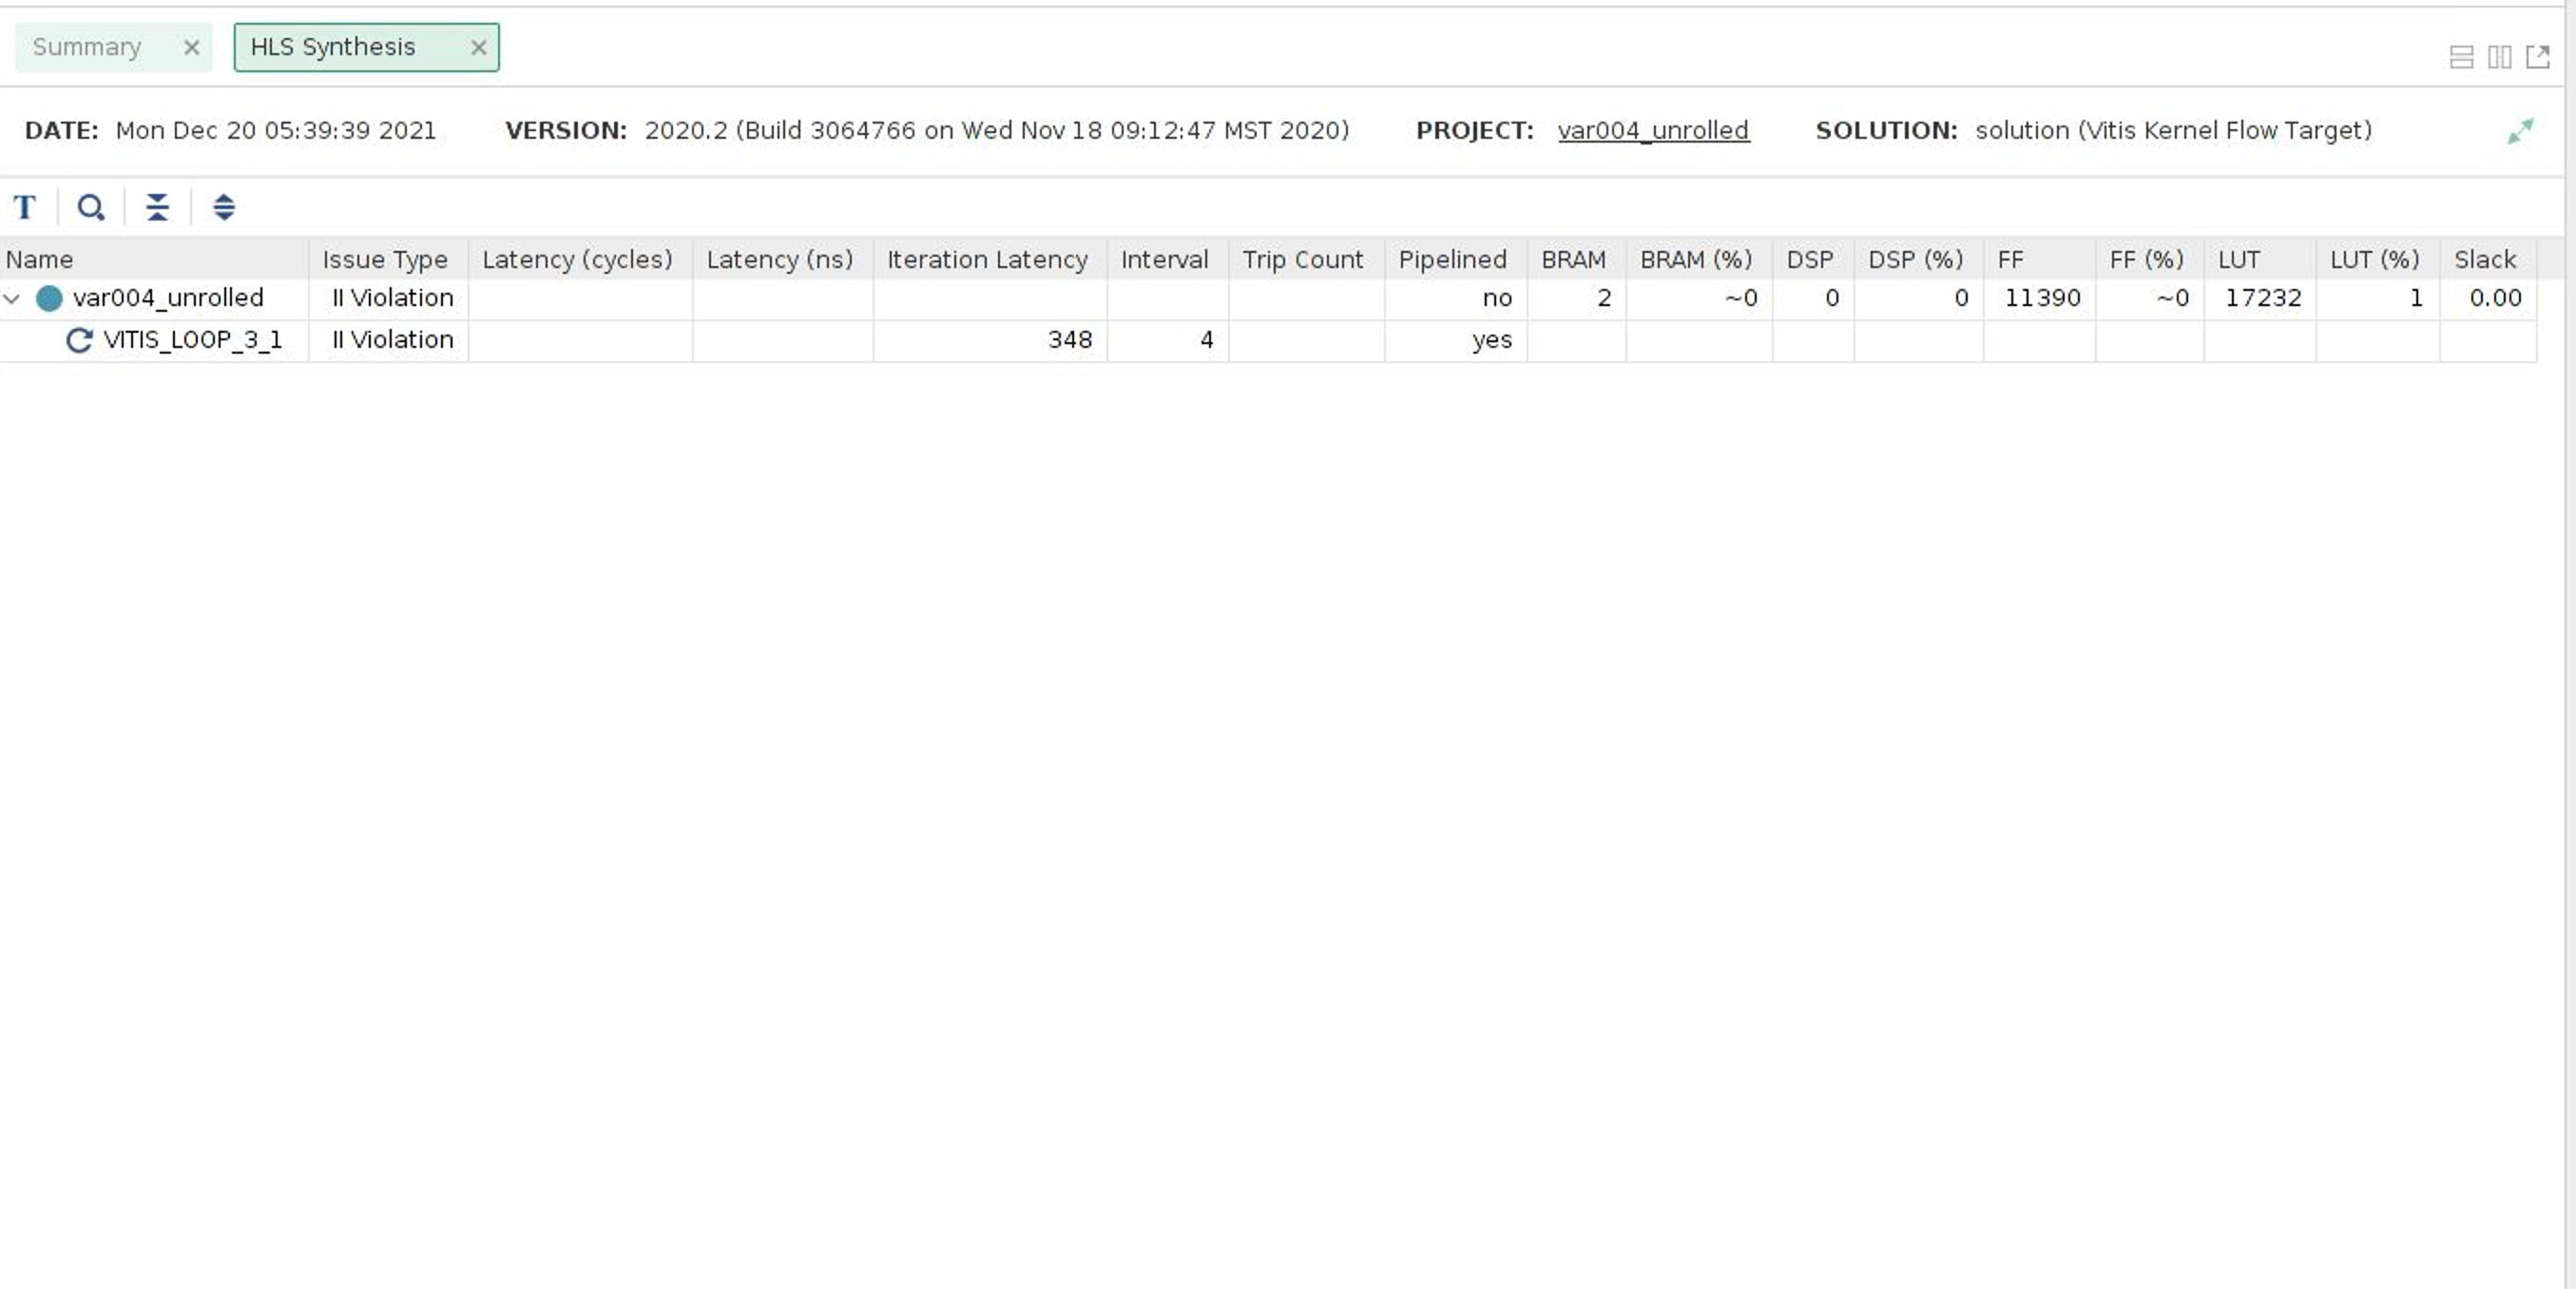
\includegraphics[width = \linewidth]{syn_unrolled.png}
	\caption{Копия экрана для вкладки «HLS Synthesis» для ядра с частично развернутым циклом}
	\label{img:syn_unrolled}
\end{figure}
\newpage
\begin{figure}[h!p]
	\centering
	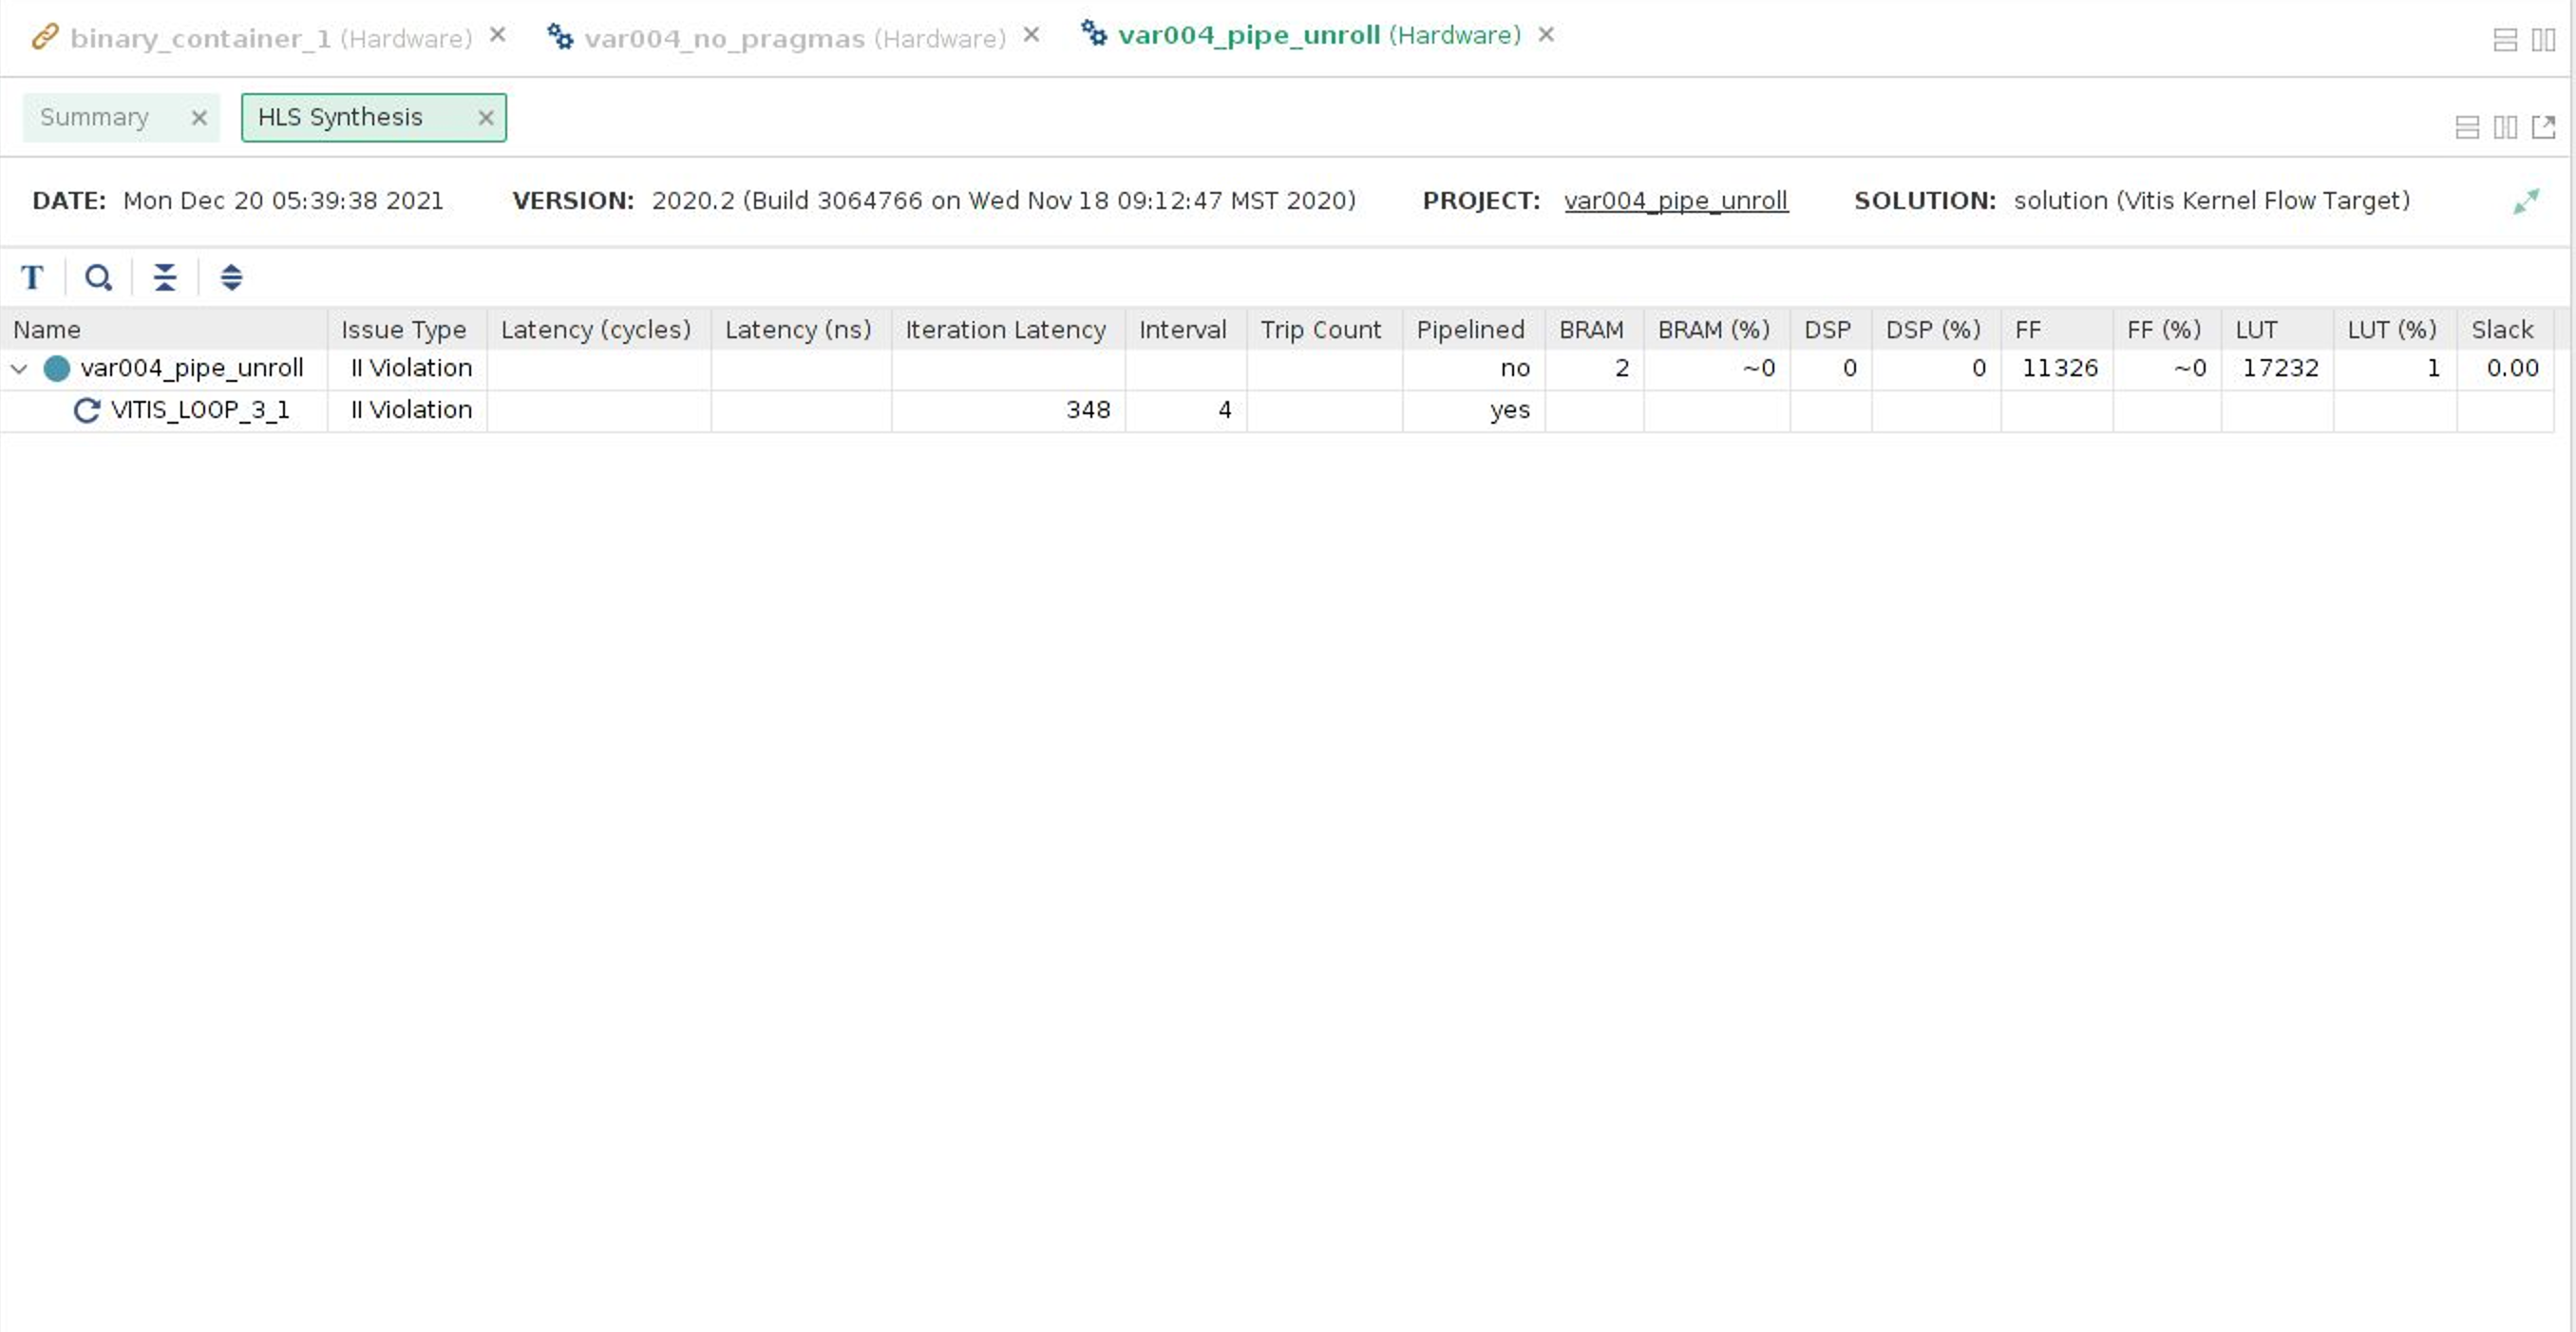
\includegraphics[width = \linewidth]{syn_pipe_unroll.png}
	\caption{Копия экрана для вкладки «HLS Synthesis» для ядра с конвейерным и частично развернутым циклом}
	\label{img:syn_pipe_unroll}
\end{figure}

В результате сборки проекта было выяснено, что самым быстрым является ядро с конвейерным, частично развернутым циклом, так как данный подход объединяет оба метода оптимизации: разворачивание циклов и конвейеризацию, а самым медленным является ядро без оптимизаций. При этом стоит отметить, что в исходном коде разворачивание циклов было настроено с параметром разворачивания 2, что также можно увидеть в полученных результатах: время выполнения развернутого цикла примерно в 2 раза быстрее, чем обычного. Конвейеризация же за счёт вложенного цикла и зависимости итераций по данным не привела к заметному повышению производительности.

\chapter*{Заключение}
\addcontentsline{toc}{chapter}{Заключение}
В ходе выполнения лабораторной работы были изучены методики и технологии синтеза аппаратных устройств ускорения вычислений по описаниям на языках высокого уровня. Также был рассмотрен маршрут проектирования устройств, представленных в виде синтаксических конструкций ЯВУ C/C++, изучены принципы работы IDE Xilinx Vitis HLS и методика анализа и отладки устройств, был разработан ускоритель вычислений по индивидуальному заданию, разработан код для тестирования ускорителя, реализован ускоритель с помощью средств высоко-уровненного синтеза, выполнена его отладка.

\chapter*{Ответы на контрольные вопросы}
\addcontentsline{toc}{chapter}{Ответы на контрольные вопросы}
\textbf{1. Назовите преимущества и недостатки аппаратных ускорителей на ПЛИС по сравнению с CPU и графическими ускорителями?}
    
CPU более универсален и подходит для самых разнообразных задач, но ввиду своей архитектуры CPU не столь эффективны для параллельных вычислений. Графические процессоры более приспособлены для целей параллельных вычислений, но работают в основном в нише отображения информации на экране. Аппаратные ускорители на ПЛИС в отличие от универсального и графического процессоров можно перепрограммировать в соответствии с особенностями решаемой на них вычислительной задачи. Получается синтез специализированного процессора под конкретную задачу. 


\textbf{2. Назовите основные способы оптимизации циклических конструкций ЯВУ, реализуемых в виде аппаратных ускорителей?}

Конвейерная обработка циклов, разворачивание циклов, потоковая обработка.

\textbf{3. Назовите этапы работы программной части ускорителя в хост системе?}

Этап 1: Инициализируется среда OpenCL. На этом этапе хост должен инициировать доступ к подключенному устройство Xilinx, и загрузить в него двоичный файл .xclbin. Затем создается очередь команд и объект ядра.

Этап 2. Приложение создает три буфера, необходимых для обмена данными с ядром: два буфера для передачи исходных данных и один для вывода результата (память должна быть выделена с выравниванием 4 КБ). Это делается с помощью конструктора cl::Buffer, после чего буфер должен быть сопоставлен с локальной памятью ядра. Такое сопоставление производится при вызове методов setArg().

Этап 3. Запуск задачи на исполнение. Хост-программа устанавливает аргументы ядра через вызов setArg(), затем посылает команду на выполнение и читает результаты обратно в память хоста (ОЗУ хост-системы). Эти операции помещаются в очередь команд, объявленную на этапе 1. Указанные вызовы функций не являются блокирующими, а соблюдение порядка выполнения гарантируется упорядоченной очередью q. Также существует возможность организовать очередь с переупорядочиванием команд, что позволит реализовать выполнение команд по готовности ядра, а не по их порядку в очереди. Вызов q.finish() позволяет ожидать завершения всех поставленных в очередь команд.

Этап 4: После завершения работы всех команд выходной буфер Rbuf содержит результаты работы ядра. Его чтение было выполнено в конце работы вызовом метода q.enqueueMigrate-MemObjects(). После этого результаты работы могут читаться как обычный массив.

\textbf{4. В чем заключается процесс отладки для вариантов сборки Emulation-SW, Emulation-HW и Hardware?}

Программная эмуляция (Emulation-SW) - код ядра компилируется для работы на ЦПУ хост-системы. Этот вариант сборки служит для верификации совместного исполнения кода хост-системы и кода ядра, для выявления синтаксических ошибок, выполнения отладки на уровне исходного кода ядра, проверки поведения системы.

Аппаратная эмуляция (Emulation-HW) - код ядра компилируется в аппаратную модель (RTL), которая запускается в специальном симуляторе на ЦПУ. Этот вариант сборки и запуска занимает больше времени, но обеспечивает подробное и точное представление активности ядра. Данный вариант сборки полезен для тестирования функциональности ускорителя и получения начальных оценок производительности.

Аппаратное обеспечение (Hardware) - код ядра компилируется в аппаратную модель (RTL), а затем реализуется на FPGA. В результате формируется двоичный файл xclbin, который будет работать на реальной FPGA.

\textbf{5. Какие инструменты и средства анализа результатов синтеза возможно использовать в Vitis HLS для оптимизации ускорителей?}


Для оптимизаций ускорителей могут быть использованы директивы такие, как #pragma HLS UNROLL для разворачивания циклов, #pragma HLS PIPELINE для конвейеризации. 

\end{document}
